\section{\textbf{APPENDIX RIBBON-10L CURVE}} \label{APPENDIX RIBBON-10L CURVE}


\subsection       {Plot of Ribbon-10L curve
	[\ref  {01-img-Plot of Ribbon-10L curve.pdf} ] }
\label{ssec-01-img-Plot of Ribbon-10L curve.pdf}

\subsection       {Ribbon-10L Radius of Curvature
	[\ref      {02-img-Ribbon-10L Radius of Curvature.pdf}] }
\label{ssec-02-img-Ribbon-10L Radius of Curvature.pdf}

\subsection       {Ribbon-10L Validation in LinuxCNC
	[\ref      {03-img-Ribbon-10L-Validation-in-LinuxCNC.png} ] }
\label{ssec-03-img-Ribbon-10L-Validation-in-LinuxCNC.png}

\subsection     {Ribbon-10L Direction of Travel 3D
	[\ref      {04-img-Ribbon-10L Direction of Travel 3D.pdf} ] }
\label{ssec-04-img-Ribbon-10L Direction of Travel 3D.pdf}

\subsection       {Ribbon-10L First and Second Order Taylors App
	[\ref      {05-img-Ribbon-10L-First-and-Second-Order-Taylors-Approx.pdf}] }
\label{ssec-05-img-Ribbon-10L-First-and-Second-Order-Taylors-Approx.pdf}

\subsection       {Ribbon-10L First minus Second Order Taylors App
	[\ref      {06-img-Ribbon-10L-First-minus-Second-Order-Taylors-Approx.pdf}] }
\label{ssec-06-img-Ribbon-10L-First-minus-Second-Order-Taylors-Approx.pdf}

\subsection       {Ribbon-10L Separate First Second Order Taylors App
	[\ref      {07-img-Ribbon-10L-Separation-First-and-Second-Order-Taylors-Approx.pdf} ] }
\label{ssec-07-img-Ribbon-10L-Separation-First-and-Second-Order-Taylors-Approx.pdf}

\subsection       {Ribbon-10L Separation SAL and SCL
	[\ref      {08-img-Ribbon-10L-Separation-SAL-and-SCL.pdf}] }
\label{ssec-08-img-Ribbon-10L-Separation-SAL-and-SCL.pdf}

\subsection       {Ribbon-10L Chord-error in close view 2 scales
	[\ref      {09-img-Ribbon-10L-Chord-error-in-close-view-2-scales.pdf}] }
\label{ssec-09-img-Ribbon-10L-Chord-error-in-close-view-2-scales.pdf}

\subsection       {Ribbon-10L Four Components Feedrate Limit
	[\ref      {10-img-Ribbon-10L-Four-Components-Feedrate-Limit.pdf} ] }
\label{ssec-10-img-Ribbon-10L-Four-Components-Feedrate-Limit.pdf}

\subsection    {Ribbon-10L FrateCommand FrateLimit and Curr-Frate
	[\ref      {11-img-Ribbon-10L-FrateCommand-FrateLimit-and-Curr-Frate.pdf}] }
\label{ssec-11-img-Ribbon-10L-FrateCommand-FrateLimit-and-Curr-Frate.pdf}

\subsection     {Ribbon-10L FeedRateLimit minus CurrFeedRate
	[\ref      {12-img-Ribbon-10L-FeedRateLimit-minus-CurrFeedRate.pdf} ] }
\label{ssec-12-img-Ribbon-10L-FeedRateLimit-minus-CurrFeedRate.pdf}

\subsection     {Ribbon-10L FC20-Nominal X and Y Feedrate Profiles
	[\ref      {13-img-Ribbon-10L-FC20-Nominal-X-and-Y-Feedrate-Profiles.pdf} ] }
\label{ssec-13-img-Ribbon-10L-FC20-Nominal-X-and-Y-Feedrate-Profiles.pdf}

\subsection     {Ribbon-10L FC20 Nominal Tangential Acceleration
	[\ref      {14-img-Ribbon-10L-FC20-Nominal-Tangential-Acceleration.pdf} ] }
\label{ssec-14-img-Ribbon-10L-FC20-Nominal-Tangential-Acceleration.pdf}

\subsection     {Ribbon-10L FC20 Nominal Rising S-Curve Profile
	[\ref      {15-img-Ribbon-10L-FC20-Nominal-Rising-S-Curve-Profile.pdf} ] }
\label{ssec-15-img-Ribbon-10L-FC20-Nominal-Rising-S-Curve-Profile.pdf}

\subsection     {Ribbon-10L FC20 Nominal Falling S-Curve Profile
	[\ref      {16-img-Ribbon-10L-FC20-Nominal-Falling-S-Curve-Profile.pdf}] }
\label{ssec-16-img-Ribbon-10L-FC20-Nominal-Falling-S-Curve-Profile.pdf}

\subsection       {Ribbon-10L FC10 Colored Feedrate Profile ngcode
	[\ref      {17-img-Ribbon-10L-FC10-Colored-Feedrate-Profile-data_ngcode.png} ] }
\label{ssec-17-img-Ribbon-10L-FC10-Colored-Feedrate-Profile-data_ngcode.png}

\subsection       {Ribbon-10L FC20 Colored Feedrate Profile ngcode
	[\ref      {18-img-Ribbon-10L-FC20-Colored-Feedrate-Profile-data_ngcode.png} ] }
\label{ssec-18-img-Ribbon-10L-FC20-Colored-Feedrate-Profile-data_ngcode.png}

Continue ...\\

\subsection       {Ribbon-10L FC30 Colored Feedrate Profile ngcode
	[\ref      {19-img-Ribbon-10L-FC30-Colored-Feedrate-Profile-data_ngcode.png} ] }
\label{ssec-19-img-Ribbon-10L-FC30-Colored-Feedrate-Profile-data_ngcode.png}

\subsection       {Ribbon-10L FC40 Colored Feedrate Profile ngcode
	[\ref      {20-img-Ribbon-10L-FC40-Colored-Feedrate-Profile-data_ngcode.png} ] }
\label{ssec-20-img-Ribbon-10L-FC40-Colored-Feedrate-Profile-data_ngcode.png}

\subsection       {Ribbon-10L FC10 Tangential Acceleration
	[\ref      {21-img-Ribbon-10L-FC10-Tangential-Acceleration.pdf}] }
\label{ssec-21-img-Ribbon-10L-FC10-Tangential-Acceleration.pdf}

\subsection       {Ribbon-10L FC20 Tangential Acceleration
	[\ref      {22-img-Ribbon-10L-FC20-Tangential-Acceleration.pdf}] }
\label{ssec-22-img-Ribbon-10L-FC20-Tangential-Acceleration.pdf}

\subsection       {Ribbon-10L FC30 Tangential Acceleration
	[\ref      {23-img-Ribbon-10L-FC30-Tangential-Acceleration.pdf}] }
\label{ssec-23-img-Ribbon-10L-FC30-Tangential-Acceleration.pdf}

\subsection       {Ribbon-10L FC40 Tangential Acceleration
	[\ref      {24-img-Ribbon-10L-FC40-Tangential-Acceleration.pdf}] }
\label{ssec-24-img-Ribbon-10L-FC40-Tangential-Acceleration.pdf}

\subsection       {Ribbon-10L FC20 Nominal Separation NAL and NCL
	[\ref      {25-img-Ribbon-10L-FC20-Nominal-Separation-NAL-and-NCL.pdf}] }
\label{ssec-25-img-Ribbon-10L-FC20-Nominal-Separation-NAL-and-NCL.pdf}

\subsection       {Ribbon-10L SAL minus SCL for FC10 FC20 FC30 FC40
	[\ref      {26-img-Ribbon-10L-Difference-SAL-minus-SCL-for-FC10-FC20-FC30-FC40.pdf}] }
\label{ssec-26-img-Ribbon-10L-Difference-SAL-minus-SCL-for-FC10-FC20-FC30-FC40.pdf}


\subsection       {Ribbon-10L FC10 FrateCmd CurrFrate X-Frate Y-Frate
	[\ref      {27-img-Ribbon-10L-FC10-FrateCmd-CurrFrate-X-Frate-Y-Frate.pdf}] }
\label{ssec-27-img-Ribbon-10L-FC10-FrateCmd-CurrFrate-X-Frate-Y-Frate.pdf}

\subsection       {Ribbon-10L FC20 FrateCmd CurrFrate X-Frate Y-Frate
	[\ref      {28-img-Ribbon-10L-FC20-FrateCmd-CurrFrate-X-Frate-Y-Frate.pdf}] }
\label{ssec-28-img-Ribbon-10L-FC20-FrateCmd-CurrFrate-X-Frate-Y-Frate.pdf}

\subsection       {Ribbon-10L FC30 FrateCmd CurrFrate X-Frate Y-Frate
	[\ref      {29-img-Ribbon-10L-FC30-FrateCmd-CurrFrate-X-Frate-Y-Frate.pdf}] }
\label{ssec-29-img-Ribbon-10L-FC30-FrateCmd-CurrFrate-X-Frate-Y-Frate.pdf}

\subsection       {Ribbon-10L FC40 FrateCmd CurrFrate X-Frate Y-Frate
	[\ref      {30-img-Ribbon-10L-FC40-FrateCmd-CurrFrate-X-Frate-Y-Frate.pdf}] }
\label{ssec-30-img-Ribbon-10L-FC40-FrateCmd-CurrFrate-X-Frate-Y-Frate.pdf}

\subsection       {Ribbon-10L FC10 Four Components FeedrateLimit
	[\ref      {31-img-Ribbon-10L-FC10-Four-Components-FeedrateLimit.pdf}] }
\label{ssec-31-img-Ribbon-10L-FC10-Four-Components-FeedrateLimit.pdf}

\subsection       {Ribbon-10L FC20 Four Components FeedrateLimit
	[\ref      {32-img-Ribbon-10L-FC20-Four-Components-FeedrateLimit.pdf}] }
\label{ssec-32-img-Ribbon-10L-FC20-Four-Components-FeedrateLimit.pdf}

\subsection       {Ribbon-10L FC30 Four Components FeedrateLimit
	[\ref      {33-img-Ribbon-10L-FC30-Four-Components-FeedrateLimit.pdf}] }
\label{ssec-33-img-Ribbon-10L-FC30-Four-Components-FeedrateLimit.pdf}

\subsection       {Ribbon-10L FC40 Four Components FeedrateLimit
	[\ref      {34-img-Ribbon-10L-FC40-Four-Components-FeedrateLimit.pdf}]}
\label{ssec-34-img-Ribbon-10L-FC40-Four-Components-FeedrateLimit.pdf}

\subsection       {Ribbon-10L Histogram Points FC10 FC20 FC30 FC40
	[\ref      {35-img-Ribbon-10L-Histogram-Points-FC10-FC20-FC30-FC40.pdf}] }
\label{ssec-35-img-Ribbon-10L-Histogram-Points-FC10-FC20-FC30-FC40.pdf}

\subsection    {Ribbon-10L Table distribution of interpolated points
	[\ref      {tab-Ribbon-10L Table distribution of interpolated points}] }
\label{ssec-tab-Ribbon-10L Table distribution of interpolated points}

\subsection         {Ribbon-10L Table FC10-20-30-40 Run Performance data
	[\ref      {tab-app4-Ribbon-10L-Table-FC10-20-30-40-Run-Performance-data}] }
\label{ssec-tab-app4-Ribbon-10L-Table-FC10-20-30-40-Run-Performance-data}


%% =====================================================
%% =====================================================
\clearpage
\pagebreak

\begin{figure}
	\caption     {Plot of Ribbon-10L curve}
	\label{01-img-Plot of Ribbon-10L curve.pdf}
	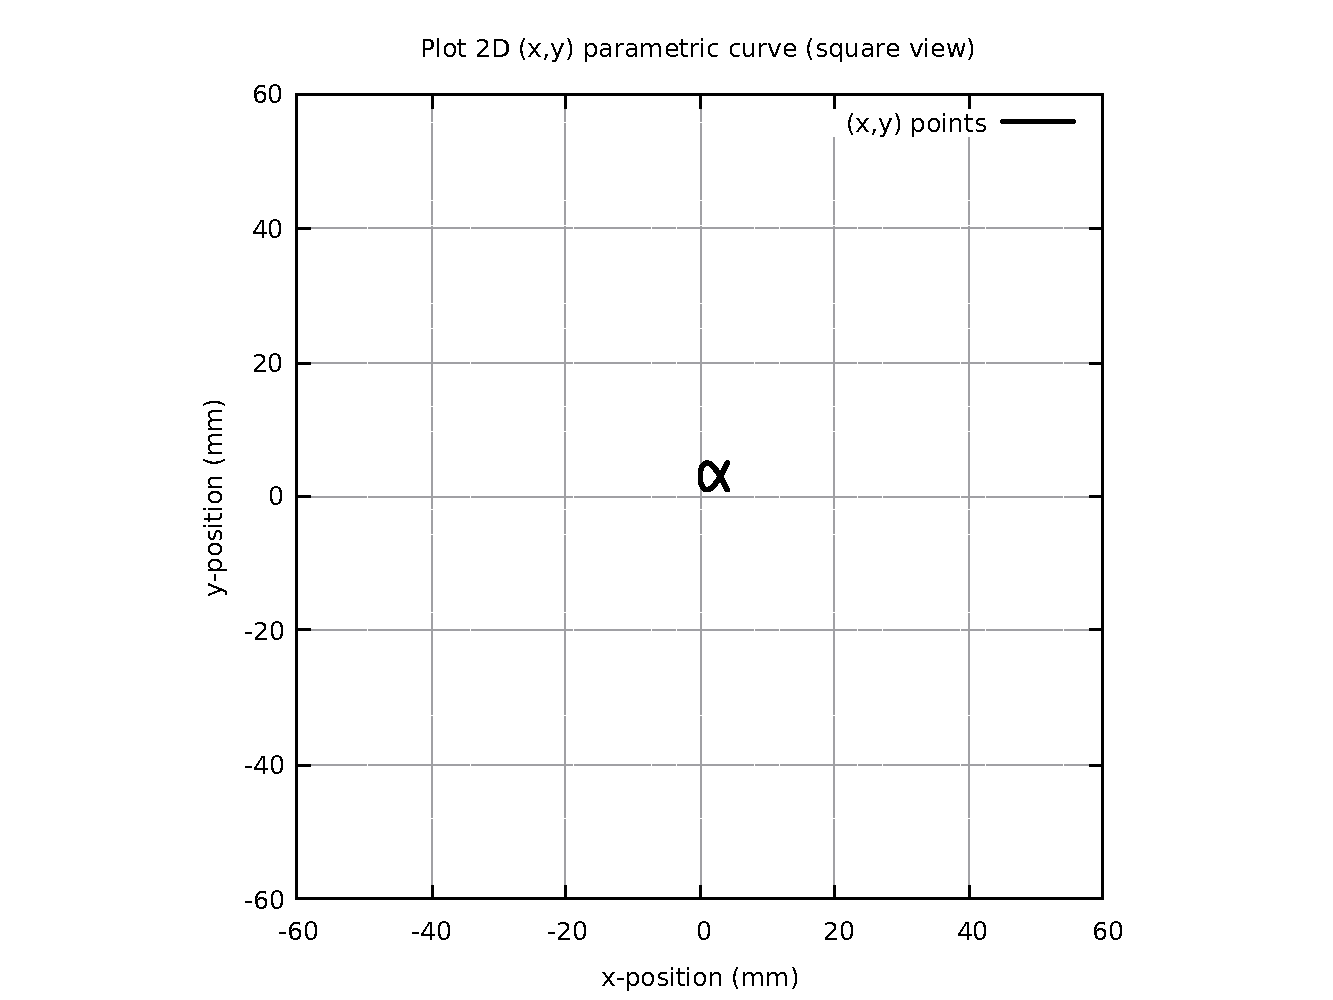
\includegraphics[width=1.00\textwidth]{Chap4/appendix/app-Ribbon-10L/plots/01-img-Plot of Ribbon-10L curve.pdf}
\end{figure}	


\begin{figure}
	\caption     {Ribbon-10L Radius of Curvature}
	\label{02-img-Ribbon-10L Radius of Curvature.pdf}
	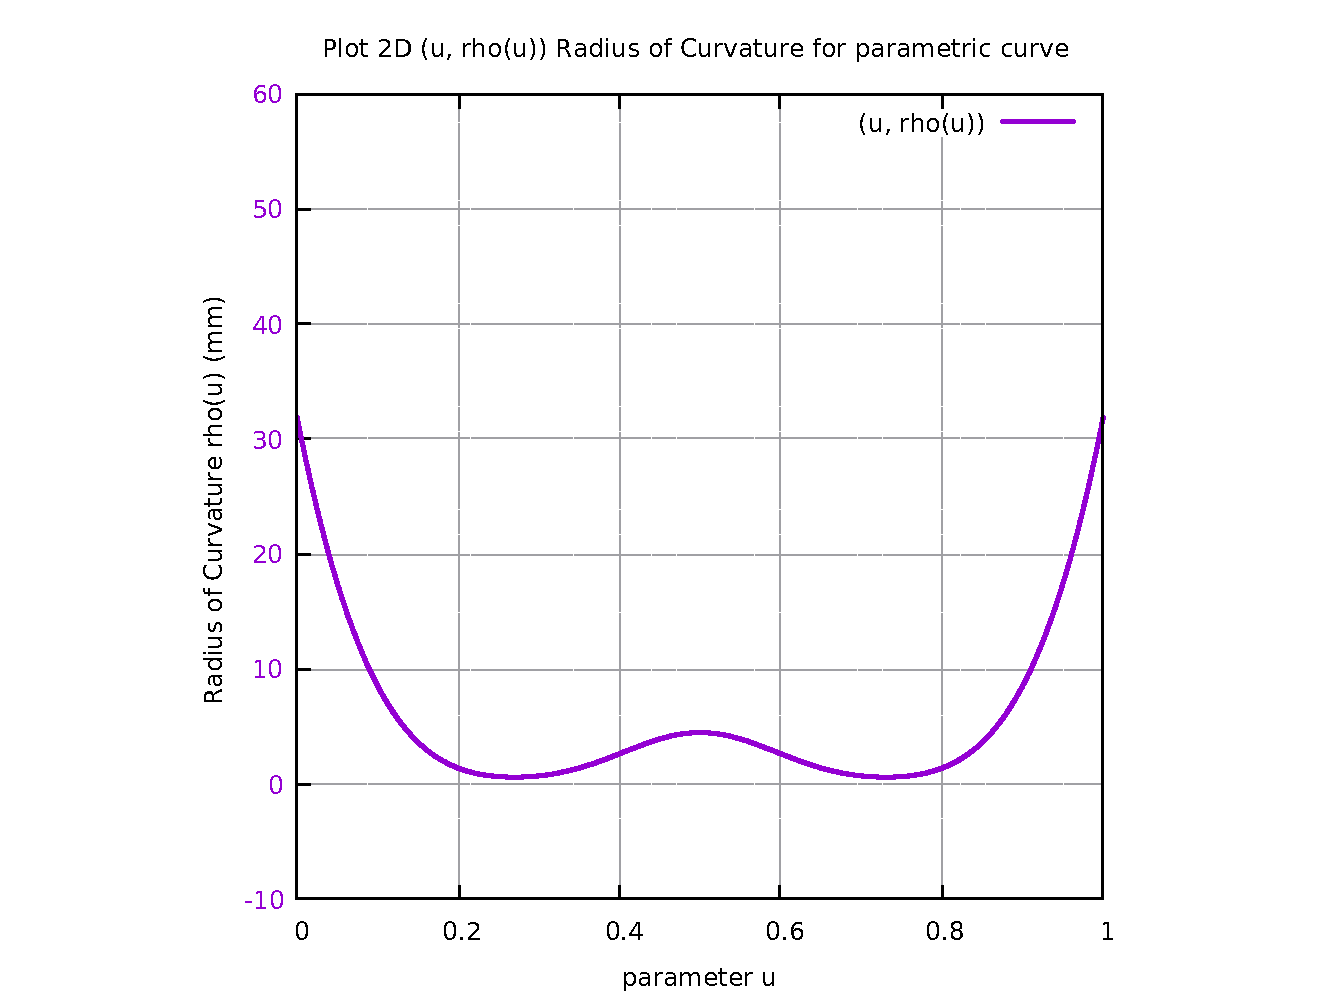
\includegraphics[width=1.00\textwidth]{Chap4/appendix/app-Ribbon-10L/plots/02-img-Ribbon-10L Radius of Curvature.pdf} 
\end{figure}	


%% ==================================================
\clearpage
\pagebreak

\begin{figure}
	\caption     {Ribbon-10L Validation in LinuxCNC}
	\label{03-img-Ribbon-10L-Validation-in-LinuxCNC.png}
	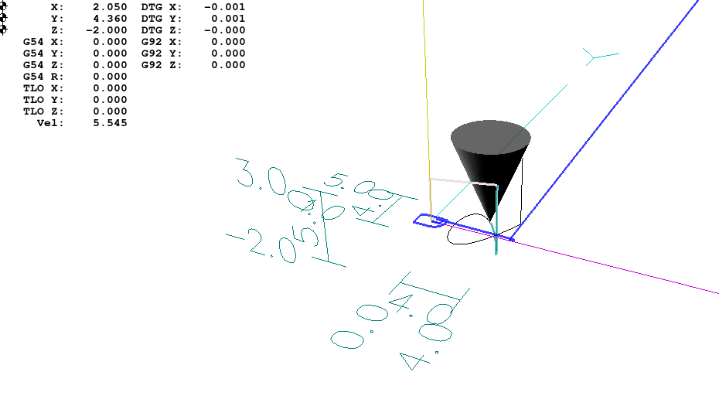
\includegraphics[width=1.00\textwidth]{Chap4/appendix/app-Ribbon-10L/plots/03-img-Ribbon-10L-Validation-in-LinuxCNC.png}
\end{figure}


\begin{figure}
	\caption     {Ribbon-10L Direction of Travel 3D}
	\label{04-img-Ribbon-10L Direction of Travel 3D.pdf}
	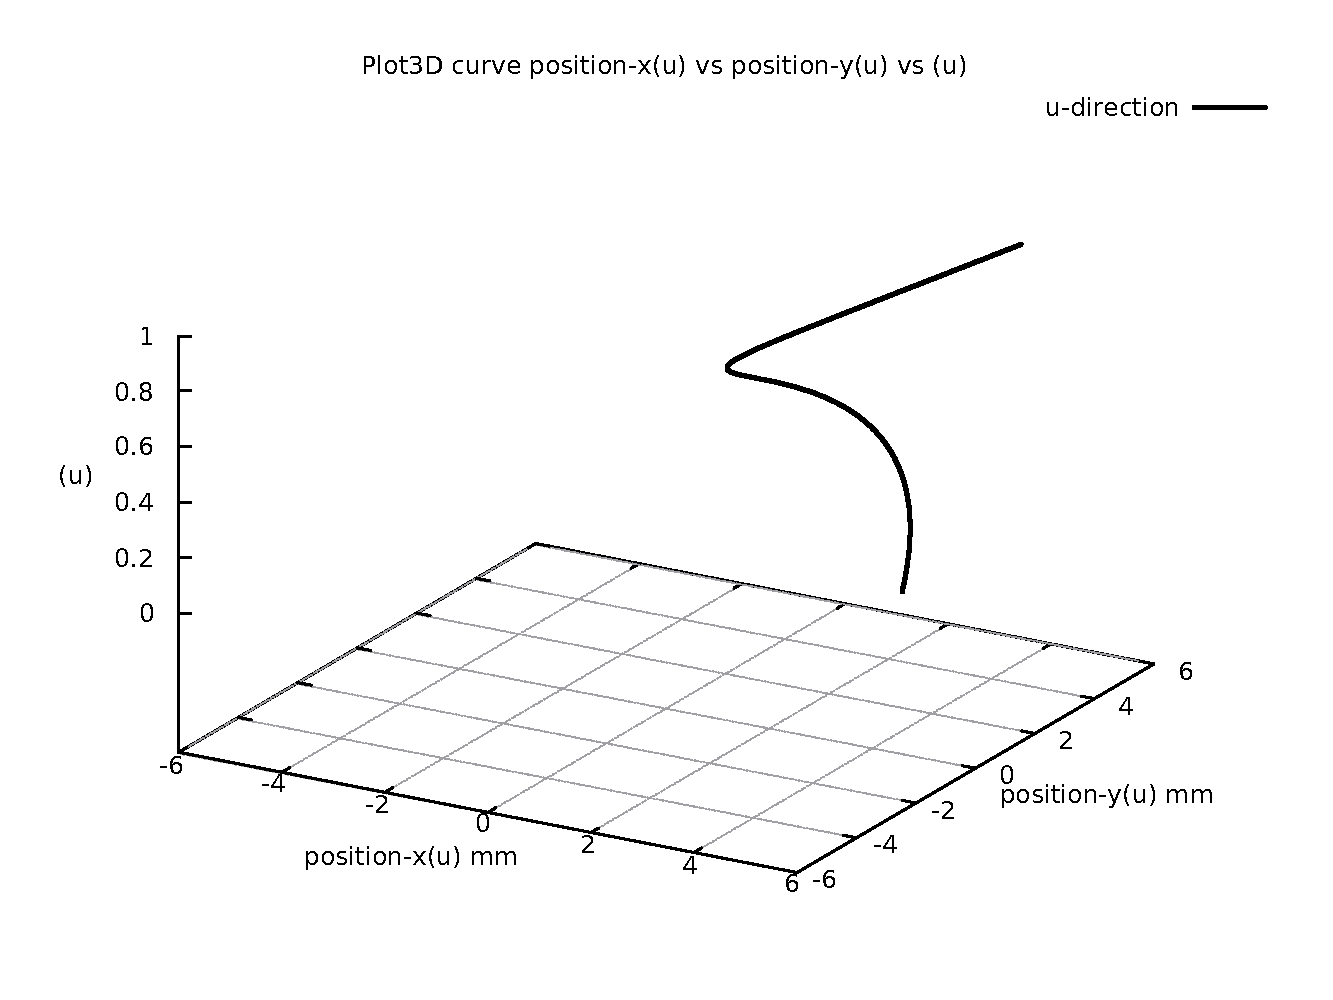
\includegraphics[width=1.00\textwidth]{Chap4/appendix/app-Ribbon-10L/plots/04-img-Ribbon-10L Direction of Travel 3D.pdf}
\end{figure}

%% ==================================================
\clearpage
\pagebreak

\begin{figure}
	\caption     {Ribbon-10L First and Second Order Taylor's Approximation}
	\label{05-img-Ribbon-10L-First-and-Second-Order-Taylors-Approx.pdf}
	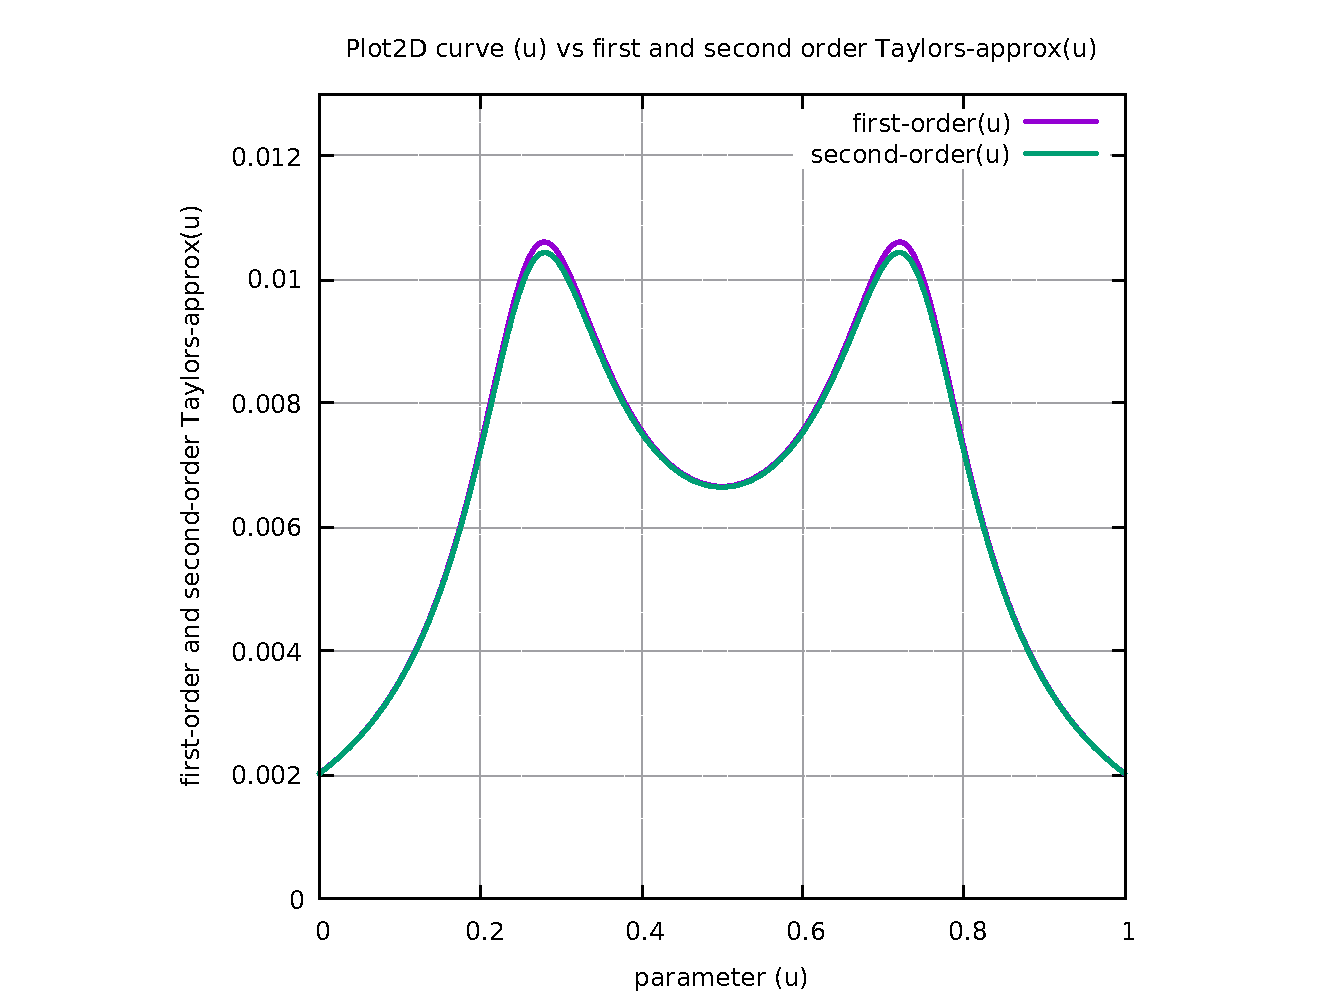
\includegraphics[width=1.00\textwidth]{Chap4/appendix/app-Ribbon-10L/plots/05-img-Ribbon-10L-First-and-Second-Order-Taylors-Approx.pdf}
\end{figure}


\begin{figure}
	\caption     {Ribbon-10L First minus Second Order Taylor's Approximation}
	\label{06-img-Ribbon-10L-First-minus-Second-Order-Taylors-Approx.pdf}
	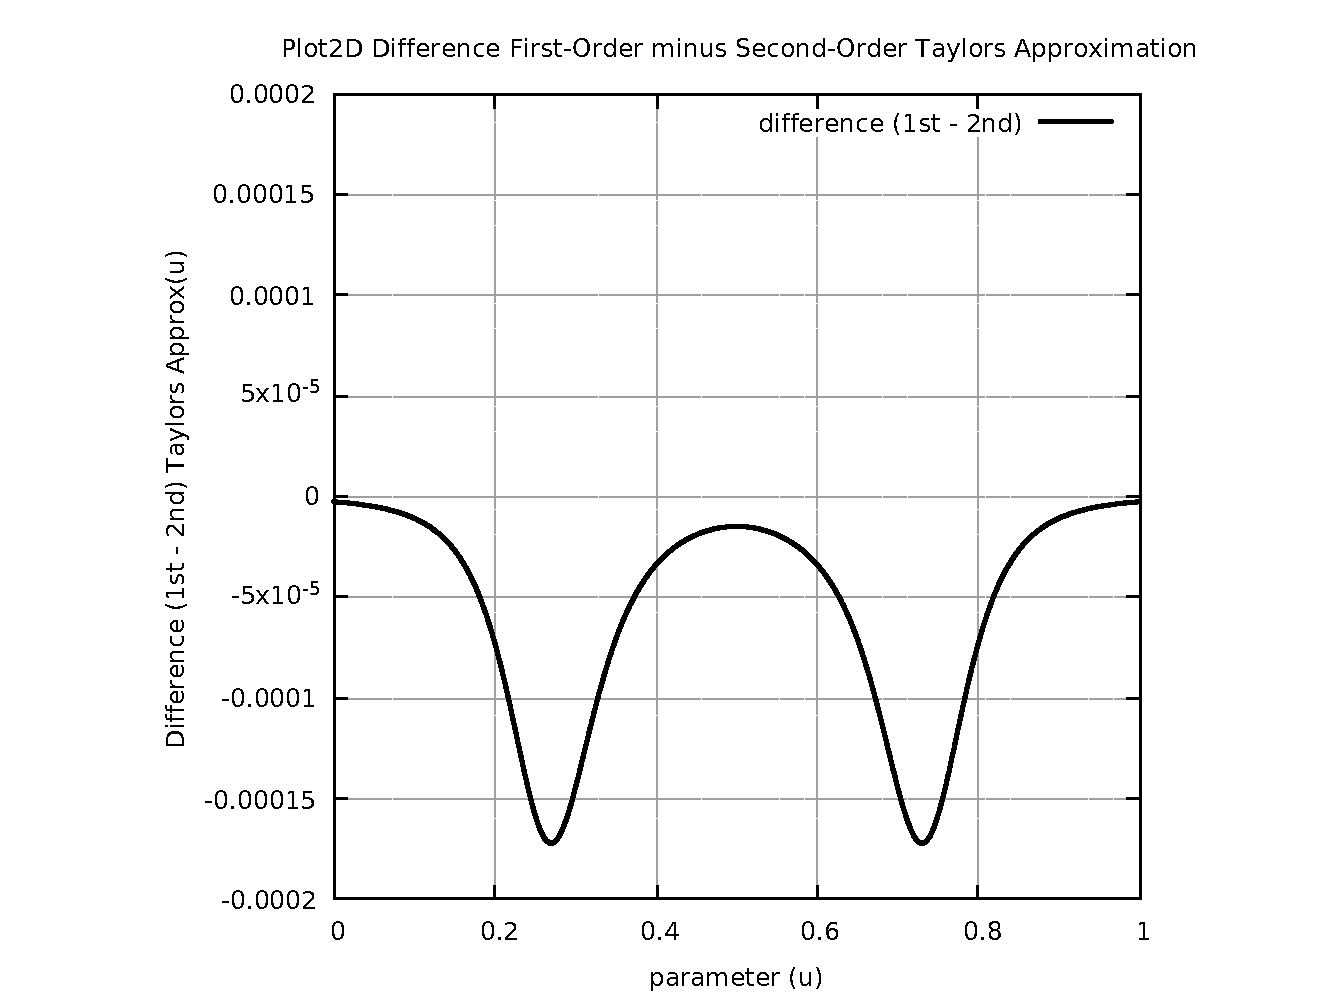
\includegraphics[width=1.00\textwidth]{Chap4/appendix/app-Ribbon-10L/plots/06-img-Ribbon-10L-First-minus-Second-Order-Taylors-Approx.pdf}
\end{figure}

%% ==================================================
\clearpage
\pagebreak

\begin{figure}
	\caption     {Ribbon-10L First and Second Order Taylor's Approximation}
	\label{07-img-Ribbon-10L-First-and-Second-Order-Taylors-Approx.pdf}
	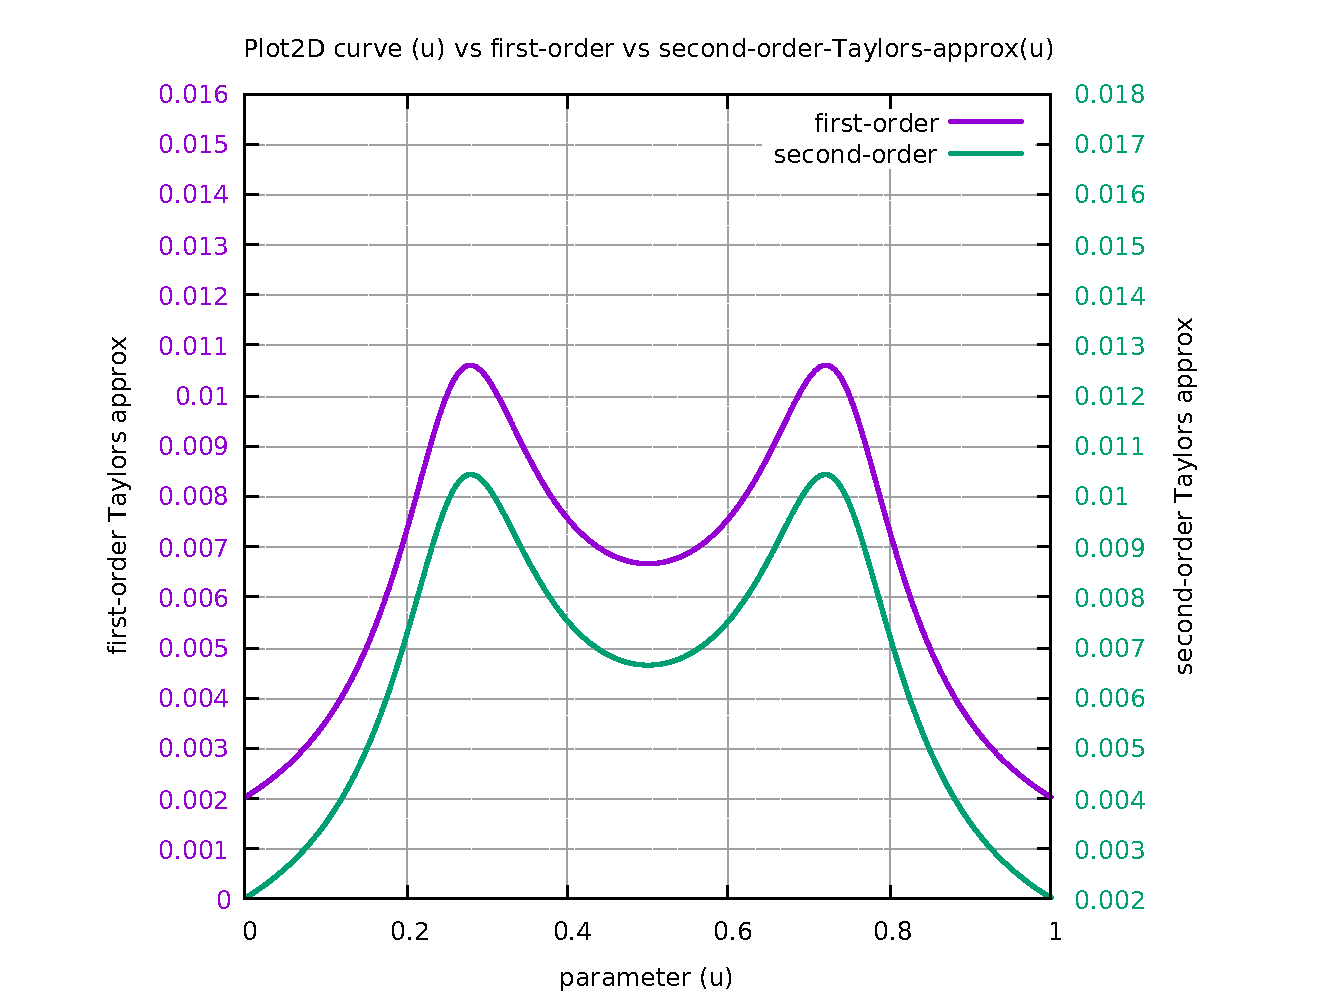
\includegraphics[width=1.00\textwidth]{Chap4/appendix/app-Ribbon-10L/plots/07-img-Ribbon-10L-First-and-Second-Order-Taylors-Approx.pdf}
\end{figure}


\begin{figure}
	\caption     {Ribbon-10L Separation SAL and SCL}
	\label{08-img-Ribbon-10L-Separation-SAL-and-SCL.pdf}
	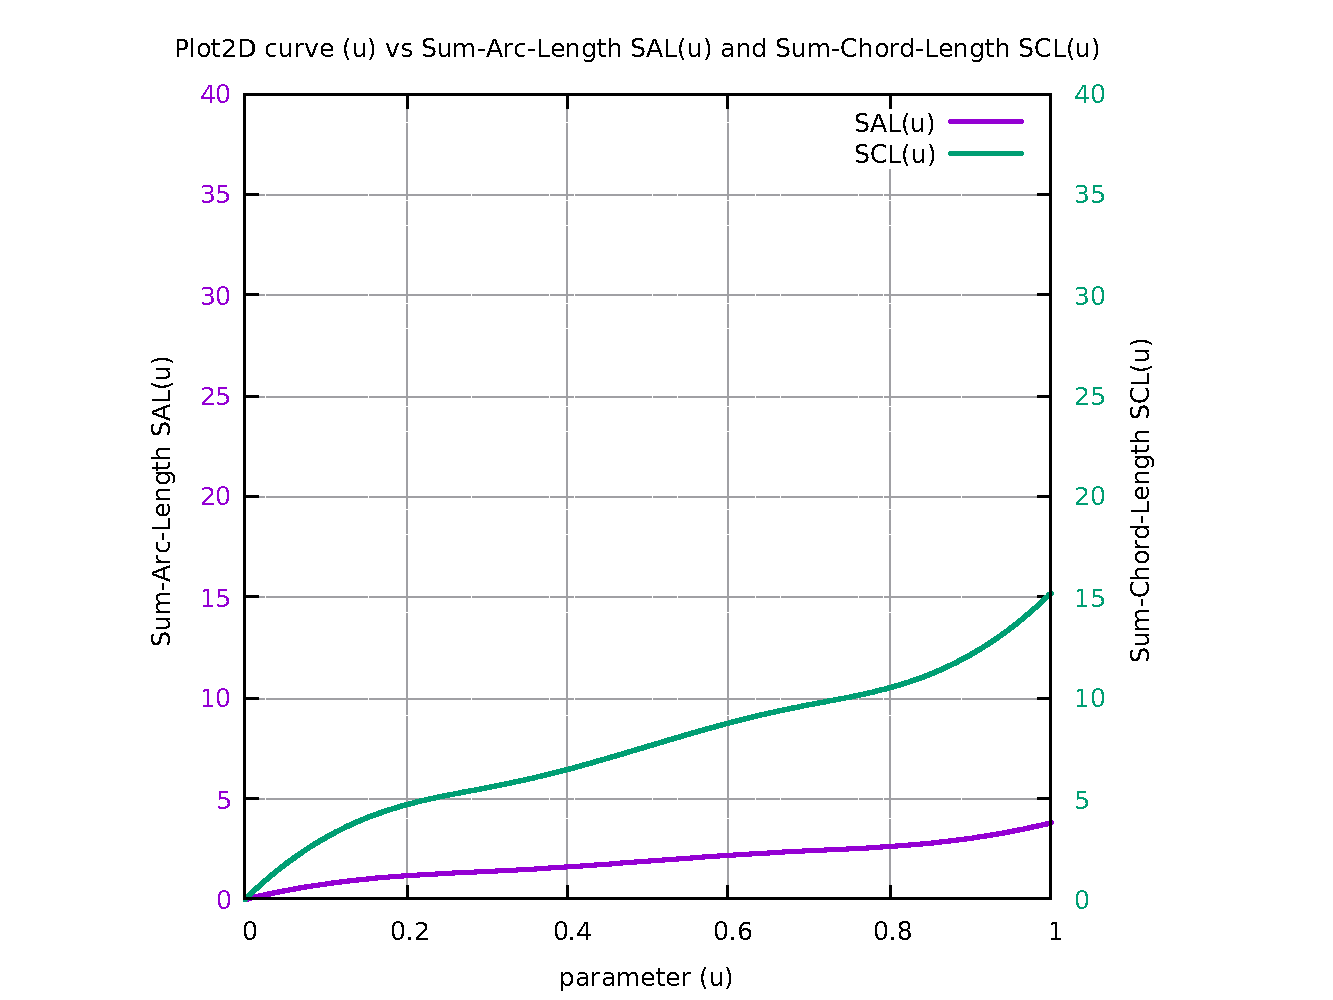
\includegraphics[width=1.00\textwidth]{Chap4/appendix/app-Ribbon-10L/plots/08-img-Ribbon-10L-Separation-SAL-and-SCL.pdf}
\end{figure}

%% ==================================================
\clearpage
\pagebreak

\begin{figure}
	\caption     {Ribbon-10L Chord-error in close view 2 scales}
	\label{09-img-Ribbon-10L-Chord-error-in-close-view-2-scales.pdf}
	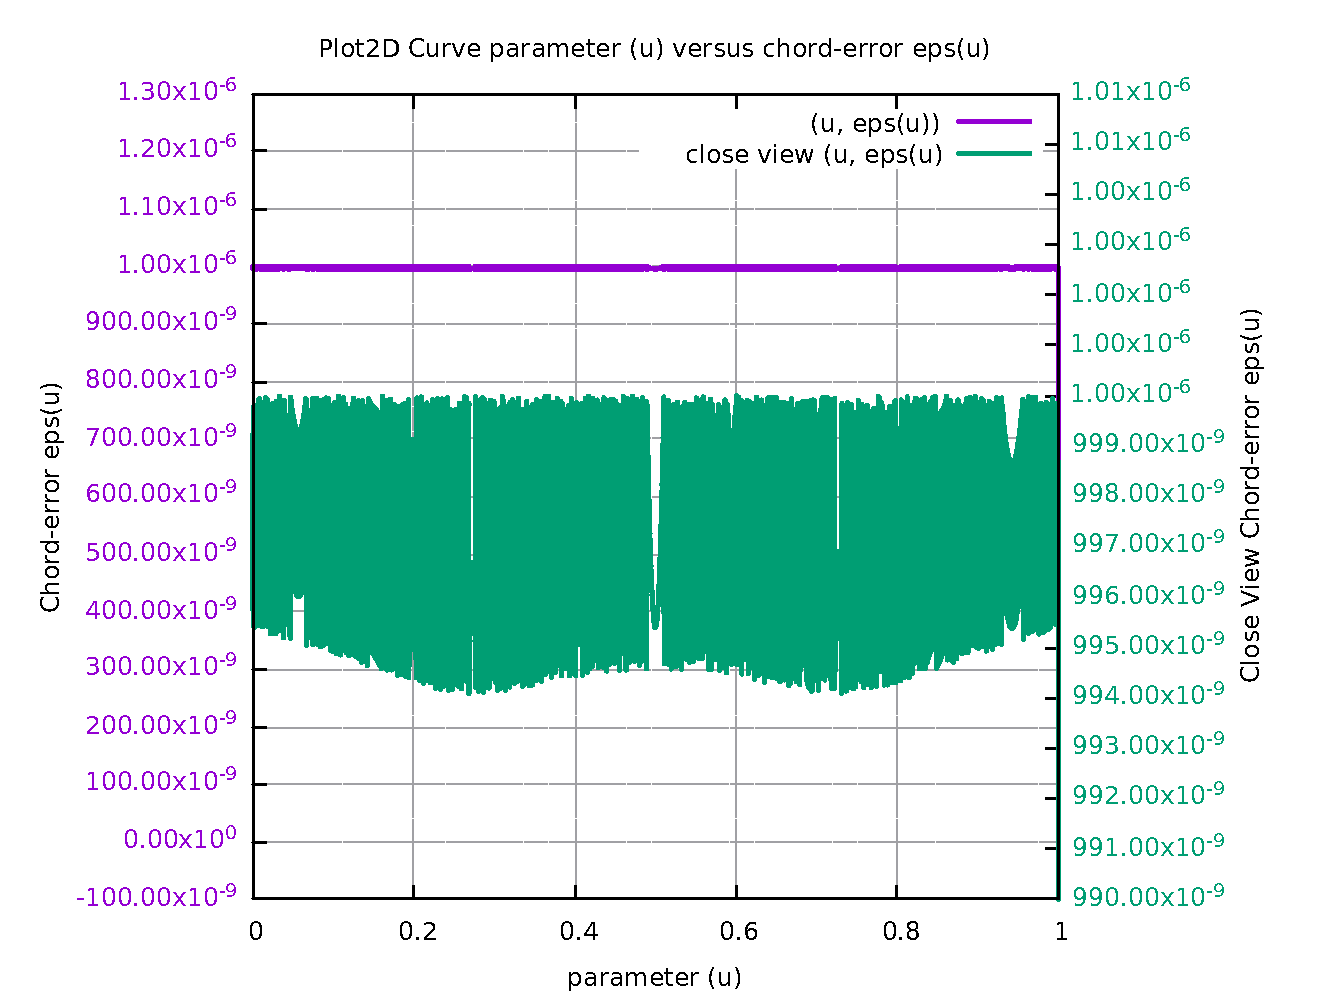
\includegraphics[width=1.00\textwidth]{Chap4/appendix/app-Ribbon-10L/plots/09-img-Ribbon-10L-Chord-error-in-close-view-2-scales.pdf}
\end{figure}

\begin{figure}
	\caption     {Ribbon-10L Four Components Feedrate Limit}
	\label{10-img-Ribbon-10L-Four-Components-Feedrate-Limit.pdf}
	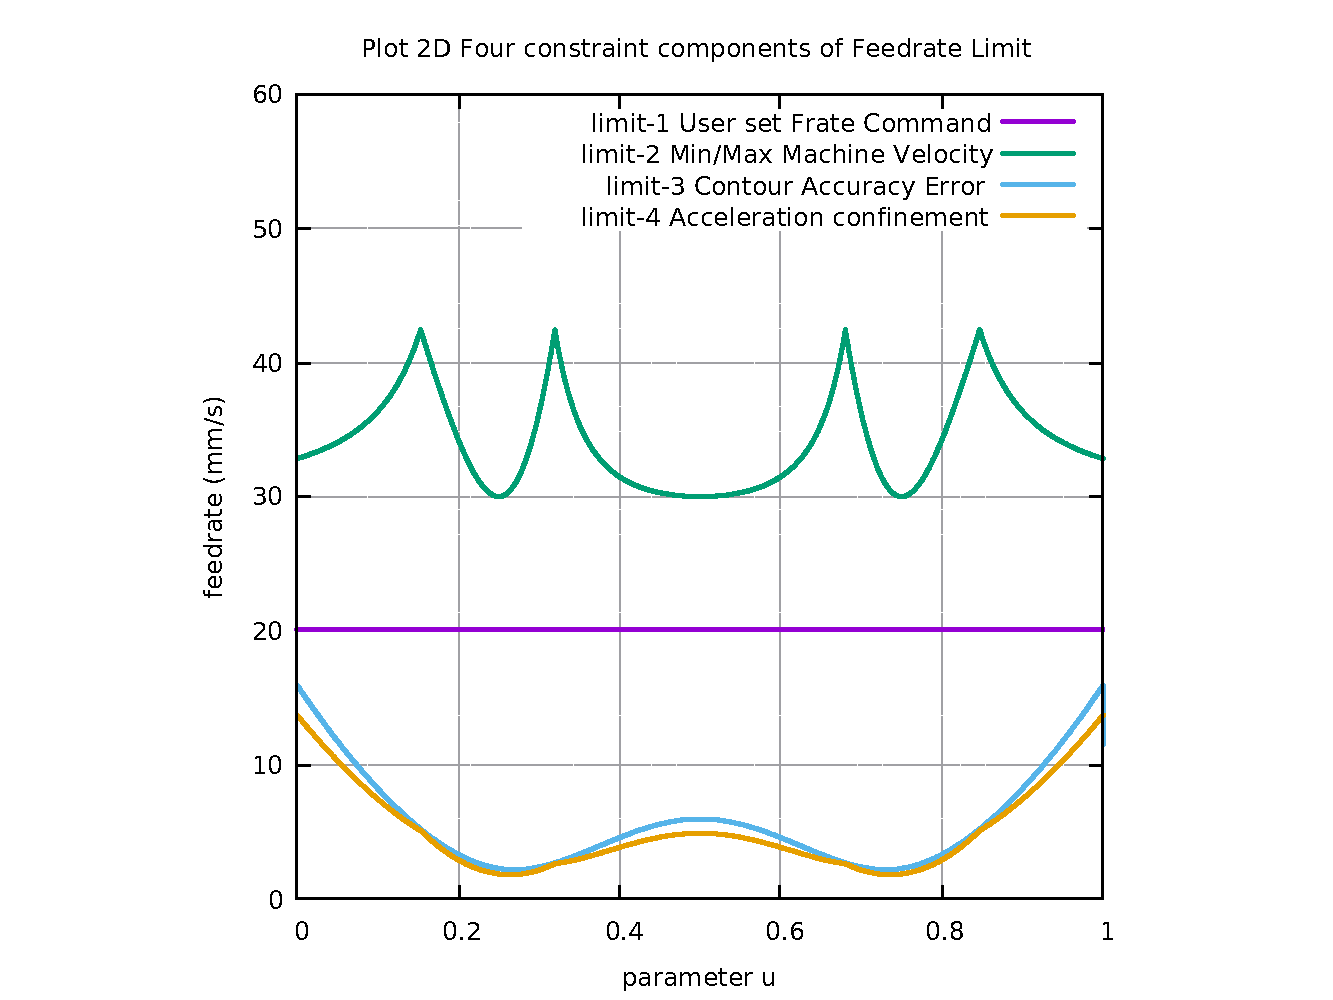
\includegraphics[width=1.00\textwidth]{Chap4/appendix/app-Ribbon-10L/plots/10-img-Ribbon-10L-Four-Components-Feedrate-Limit.pdf}
\end{figure}

%% ==================================================
\clearpage
\pagebreak

\begin{figure}
	\caption     {Ribbon-10L FrateCommand FrateLimit and Curr-Frate}
	\label{11-img-Ribbon-10L-FrateCommand-FrateLimit-and-Curr-Frate.pdf}
	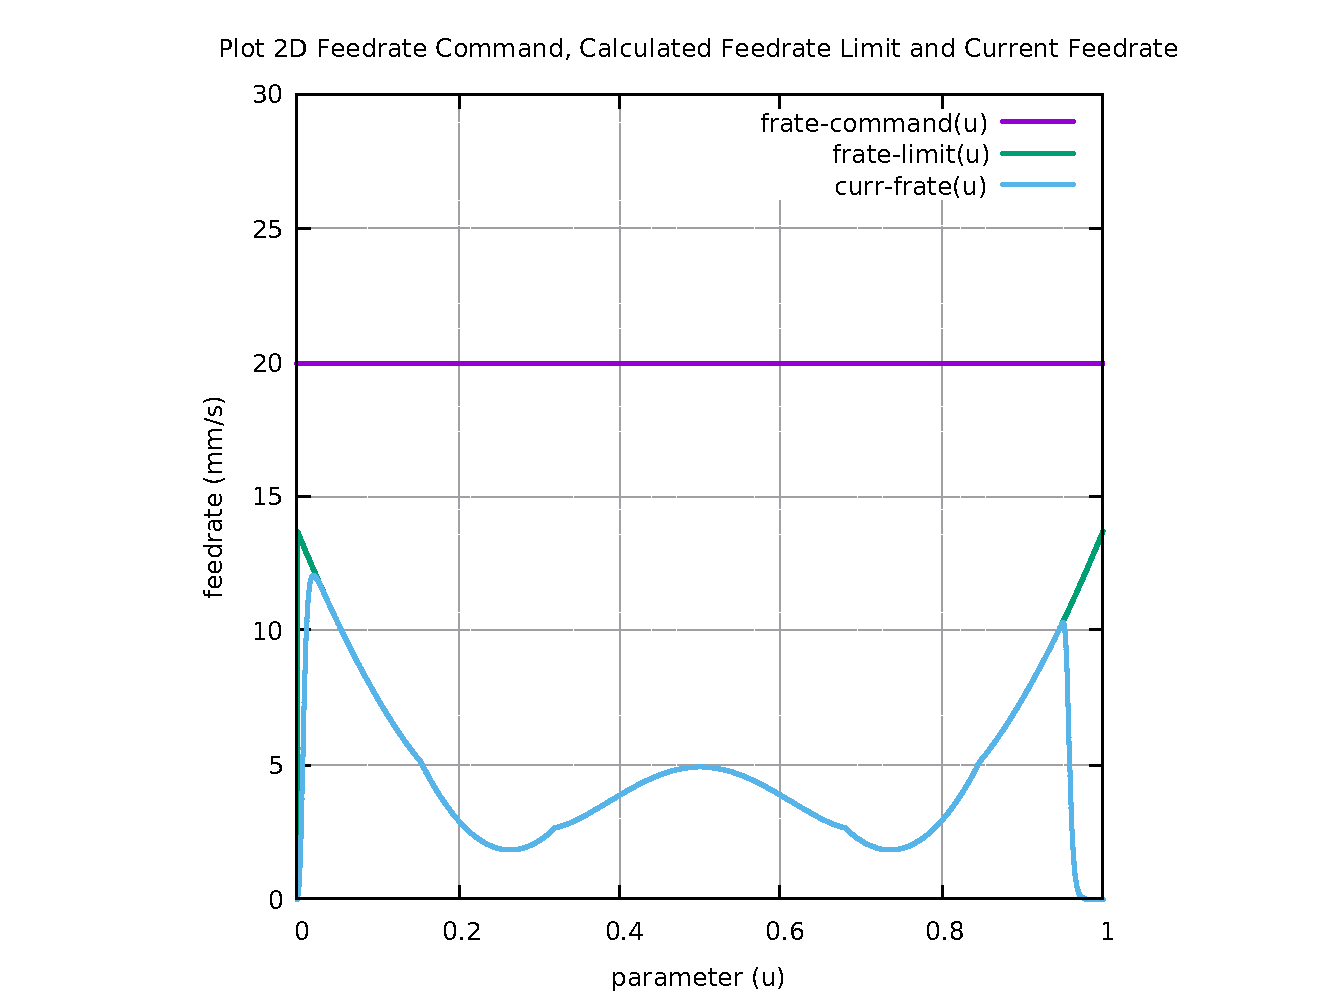
\includegraphics[width=1.00\textwidth]{Chap4/appendix/app-Ribbon-10L/plots/11-img-Ribbon-10L-FrateCommand-FrateLimit-and-Curr-Frate.pdf}
\end{figure}

\begin{figure}
	\caption     {Ribbon-10L FeedRateLimit minus CurrFeedRate}
	\label{12-img-Ribbon-10L-FeedRateLimit-minus-CurrFeedRate.pdf}
	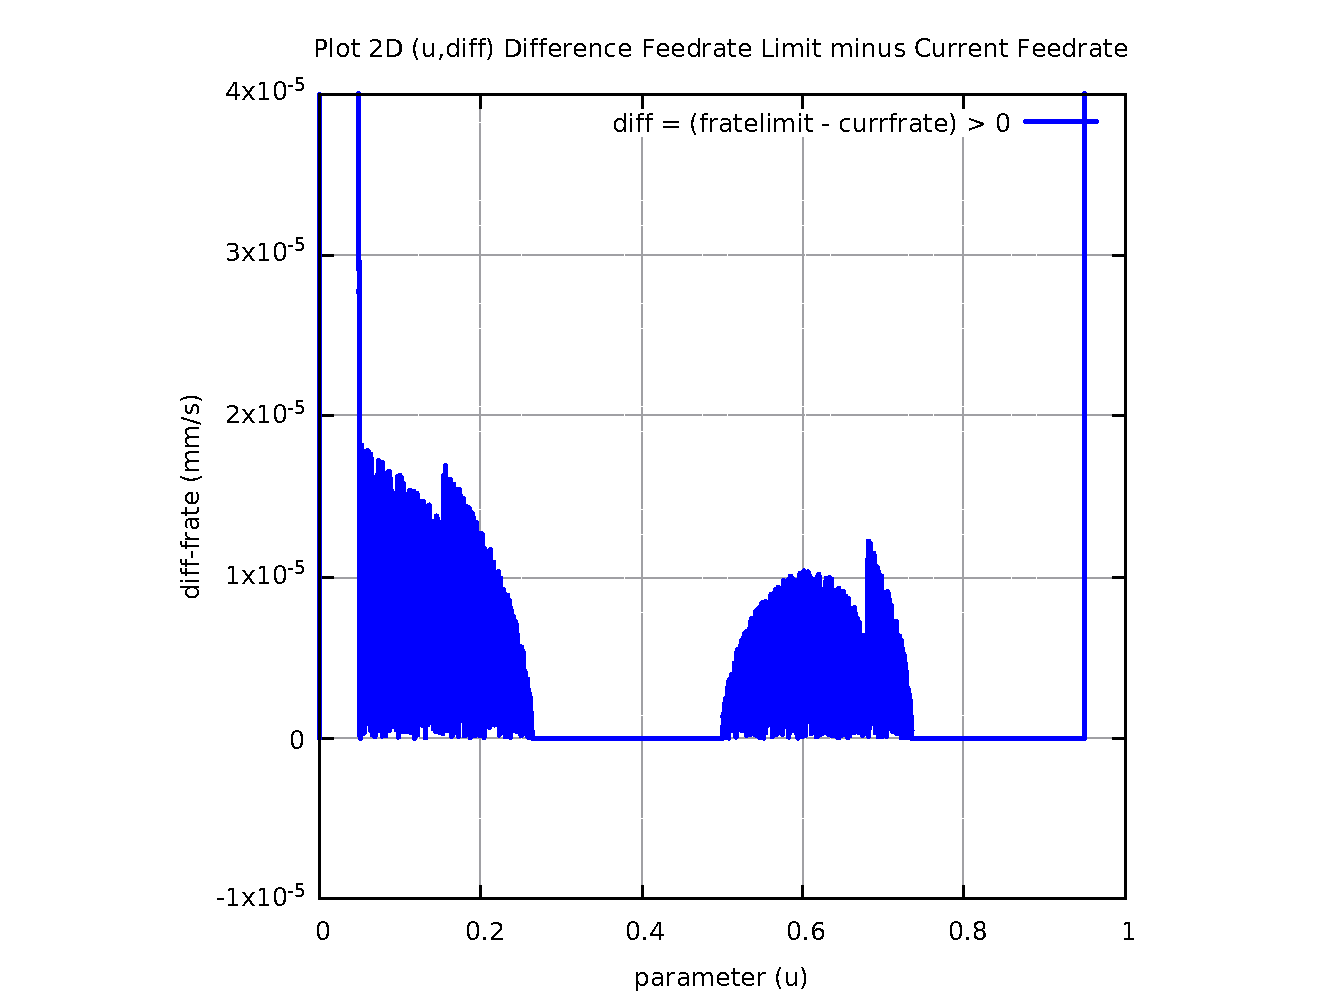
\includegraphics[width=1.00\textwidth]{Chap4/appendix/app-Ribbon-10L/plots/12-img-Ribbon-10L-FeedRateLimit-minus-CurrFeedRate.pdf}
\end{figure}

%% ==================================================
\clearpage
\pagebreak

\begin{figure}
	\caption     {Ribbon-10L FC20-Nominal X and Y Feedrate Profiles}
	\label{13-img-Ribbon-10L-FC20-Nominal-X-and-Y-Feedrate-Profiles.pdf}
	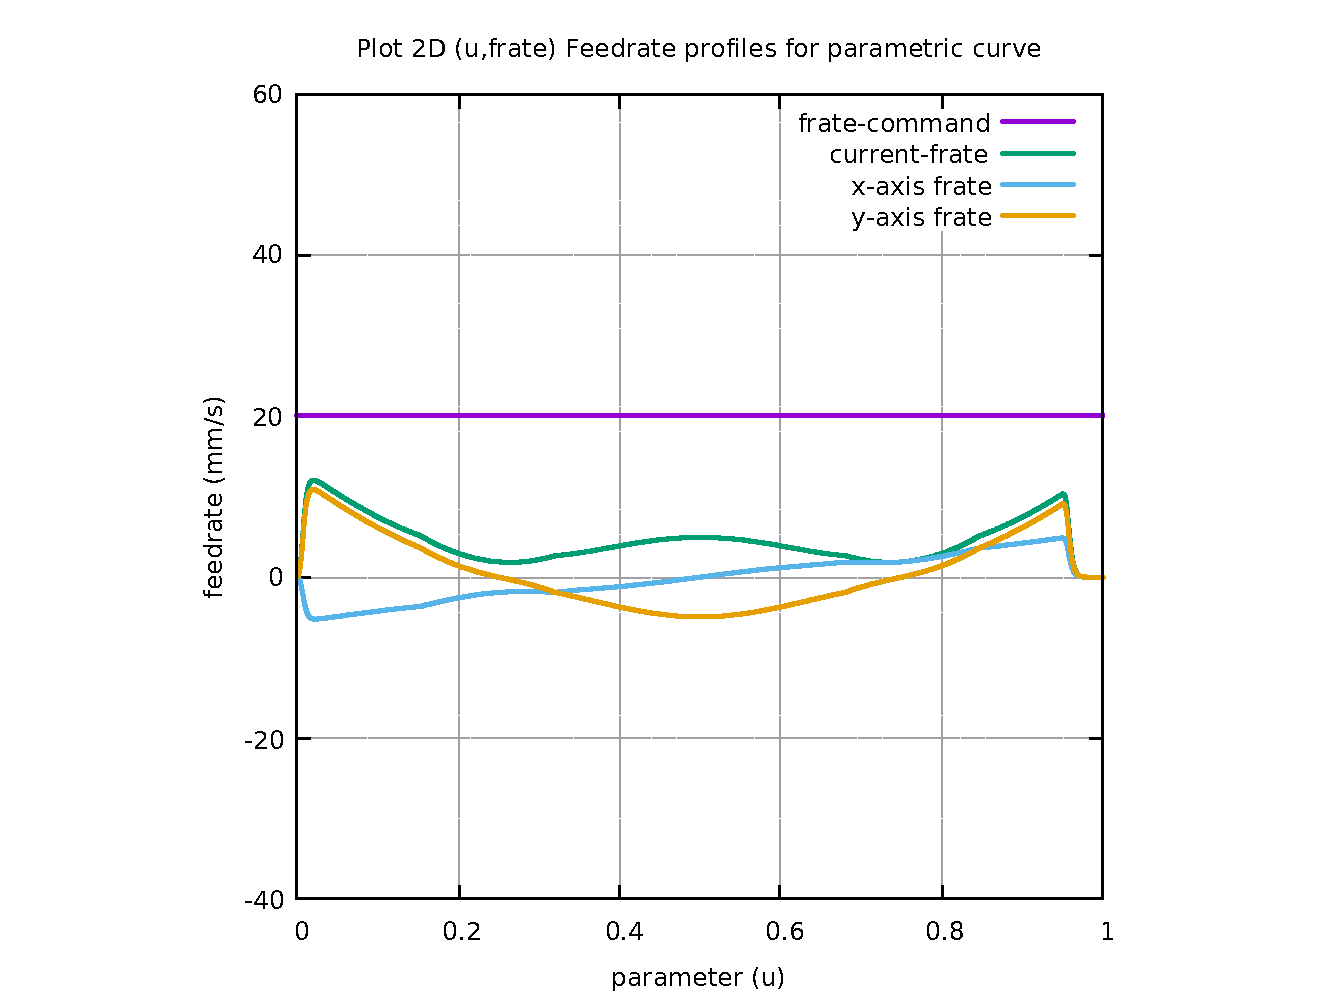
\includegraphics[width=1.00\textwidth]{Chap4/appendix/app-Ribbon-10L/plots/13-img-Ribbon-10L-FC20-Nominal-X-and-Y-Feedrate-Profiles.pdf}
\end{figure}


\begin{figure}
	\caption     {Ribbon-10L FC20 Nominal Tangential Acceleration}
	\label{14-img-Ribbon-10L-FC20-Nominal-Tangential-Acceleration.pdf}
	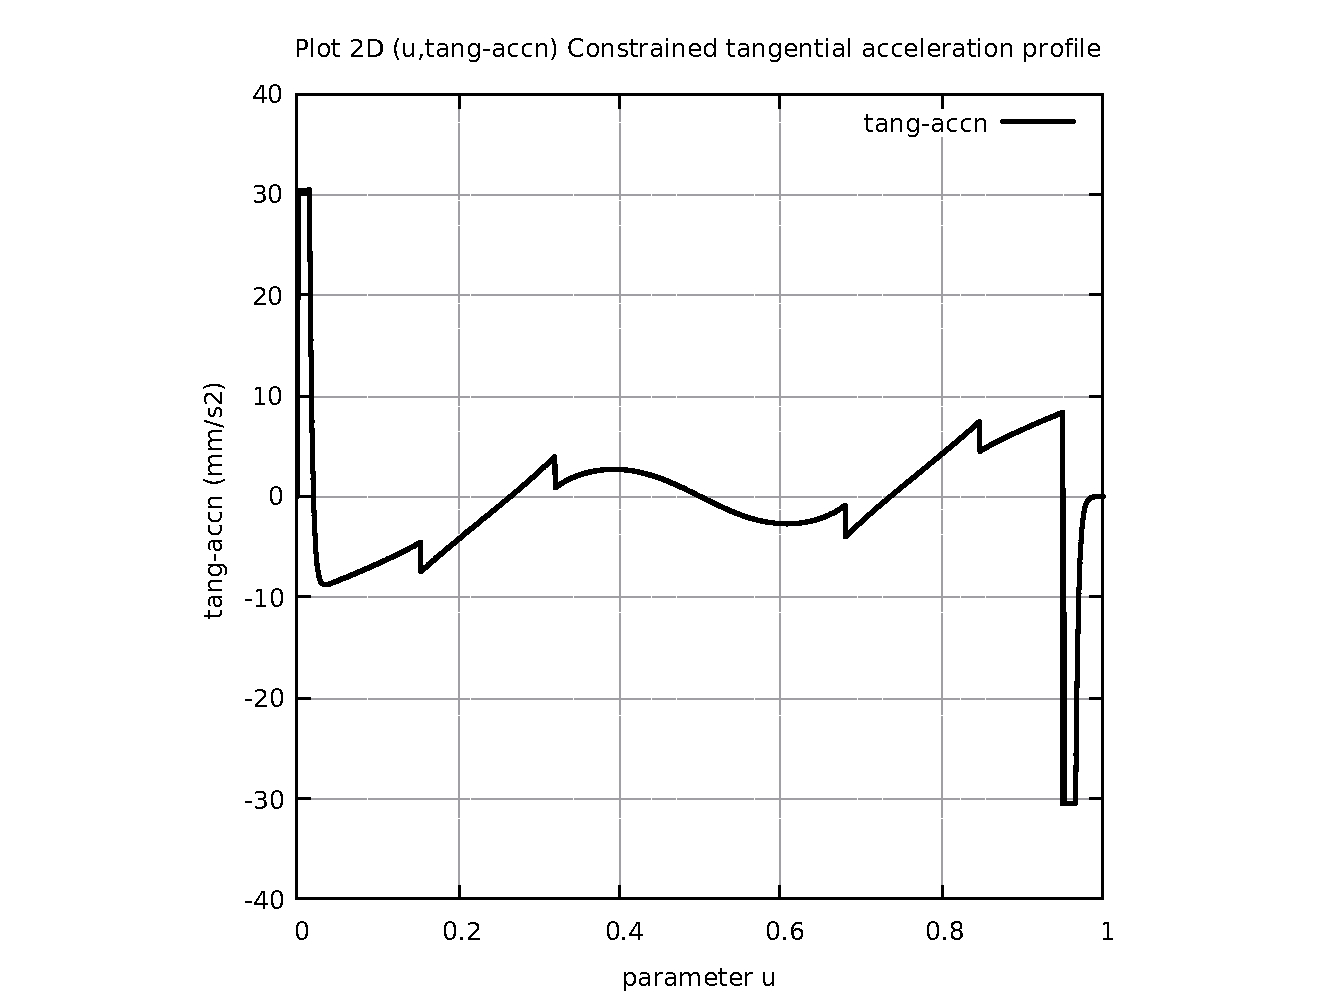
\includegraphics[width=1.00\textwidth]{Chap4/appendix/app-Ribbon-10L/plots/14-img-Ribbon-10L-FC20-Nominal-Tangential-Acceleration.pdf}
\end{figure}

%% ==================================================
\clearpage
\pagebreak

\begin{figure}
	\caption     {Ribbon-10L FC20 Nominal Rising S-Curve Profile}
	\label{15-img-Ribbon-10L-FC20-Nominal-Rising-S-Curve-Profile.pdf}
	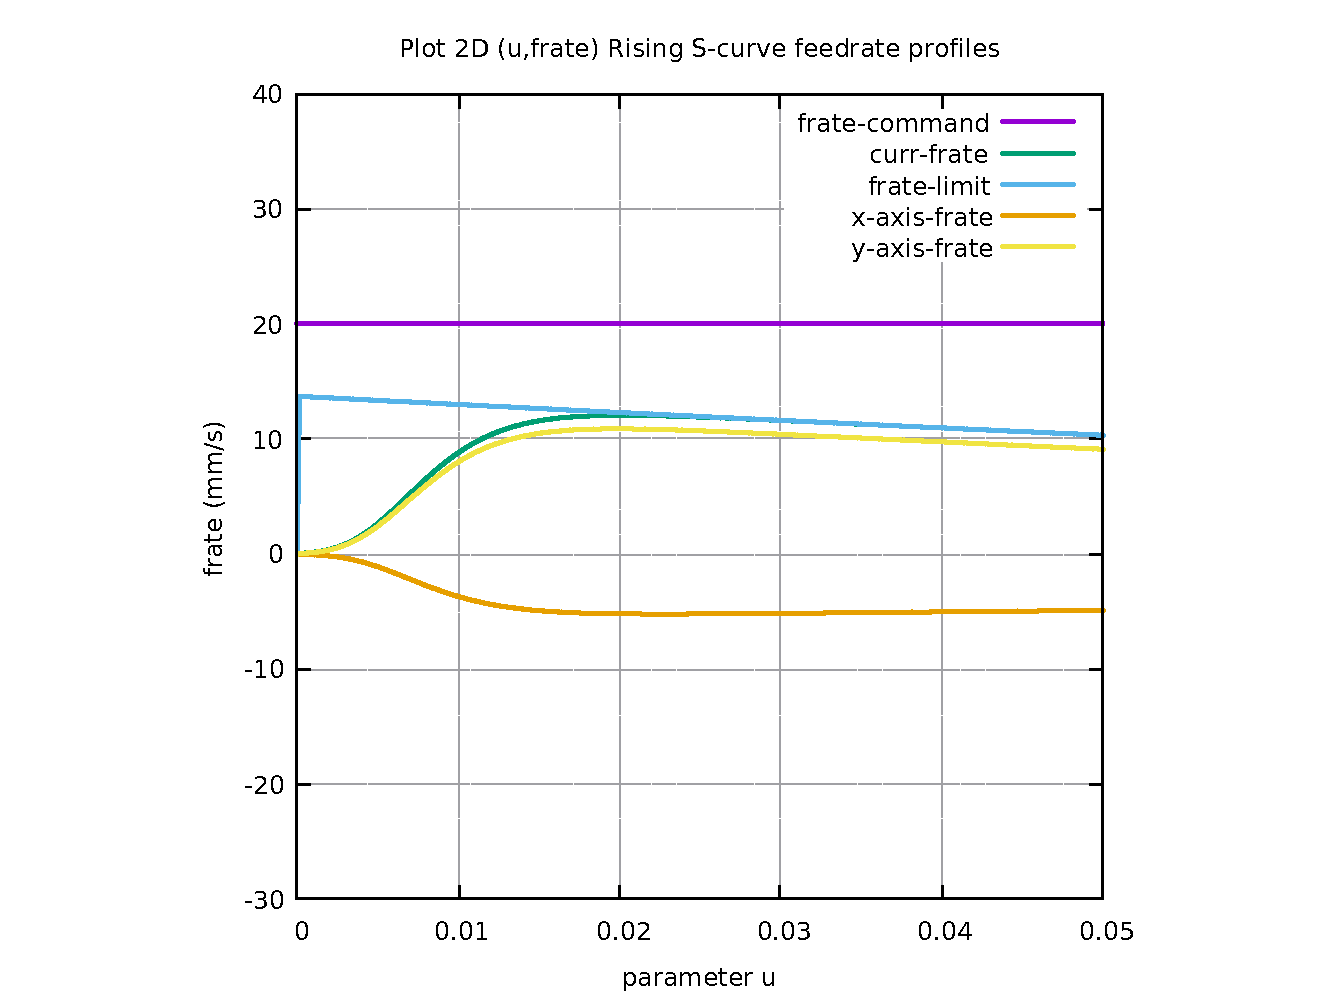
\includegraphics[width=1.00\textwidth]{Chap4/appendix/app-Ribbon-10L/plots/15-img-Ribbon-10L-FC20-Nominal-Rising-S-Curve-Profile.pdf}
\end{figure}


\begin{figure}
	\caption     {Ribbon-10L FC20 Nominal Falling S-Curve Profile}
	\label{16-img-Ribbon-10L-FC20-Nominal-Falling-S-Curve-Profile.pdf}
	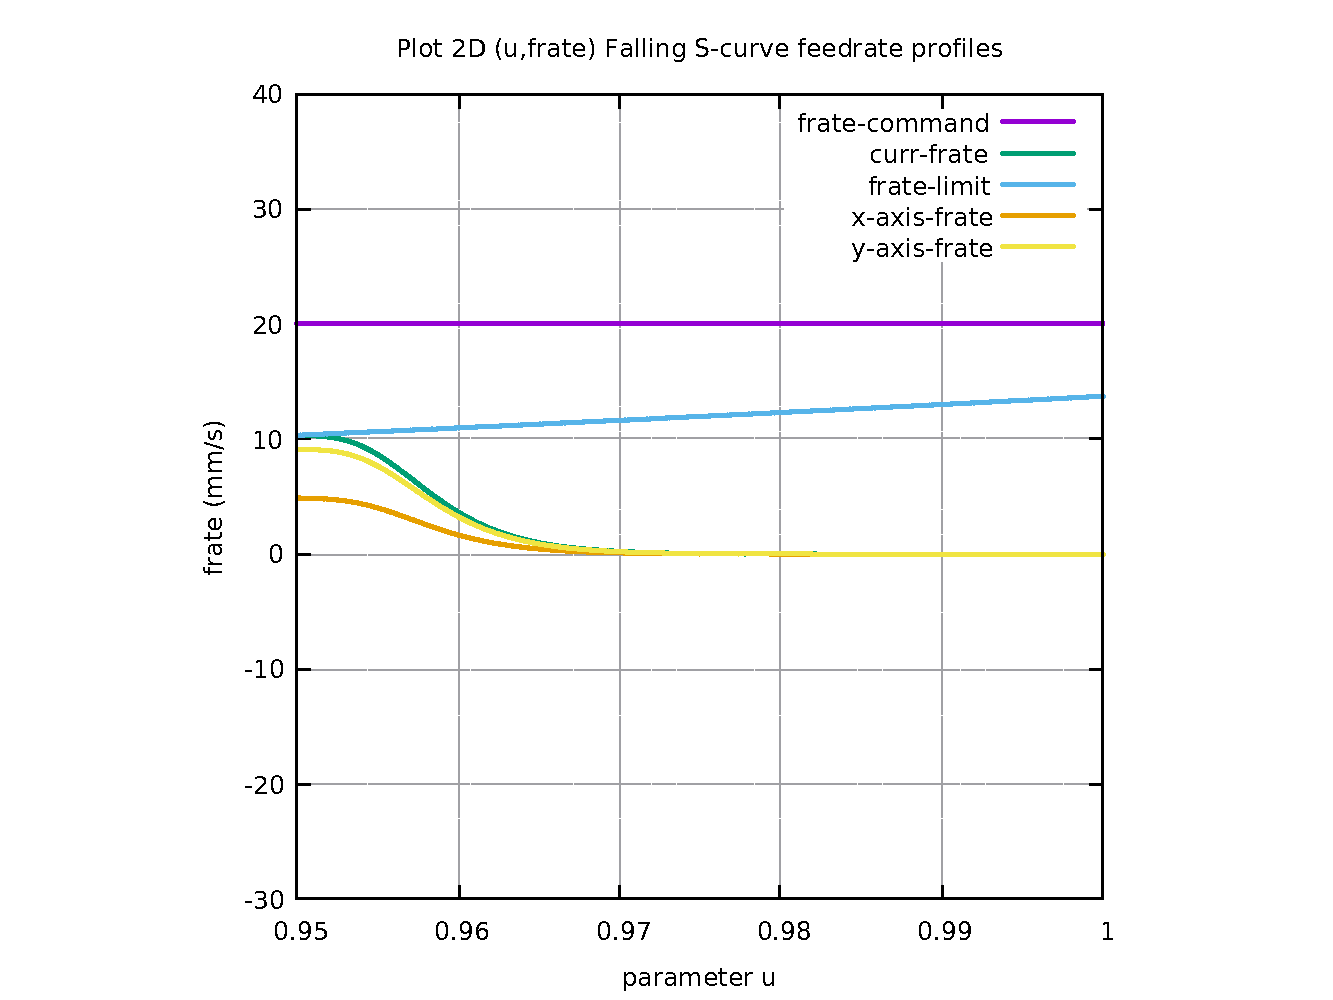
\includegraphics[width=1.00\textwidth]{Chap4/appendix/app-Ribbon-10L/plots/16-img-Ribbon-10L-FC20-Nominal-Falling-S-Curve-Profile.pdf}
\end{figure}

%% ==================================================
\clearpage
\pagebreak

\begin{figure}
	\caption     {Ribbon-10L FC10 Colored Feedrate Profile data ngcode}
	\label{17-img-Ribbon-10L-FC10-Colored-Feedrate-Profile-data_ngcode.png}
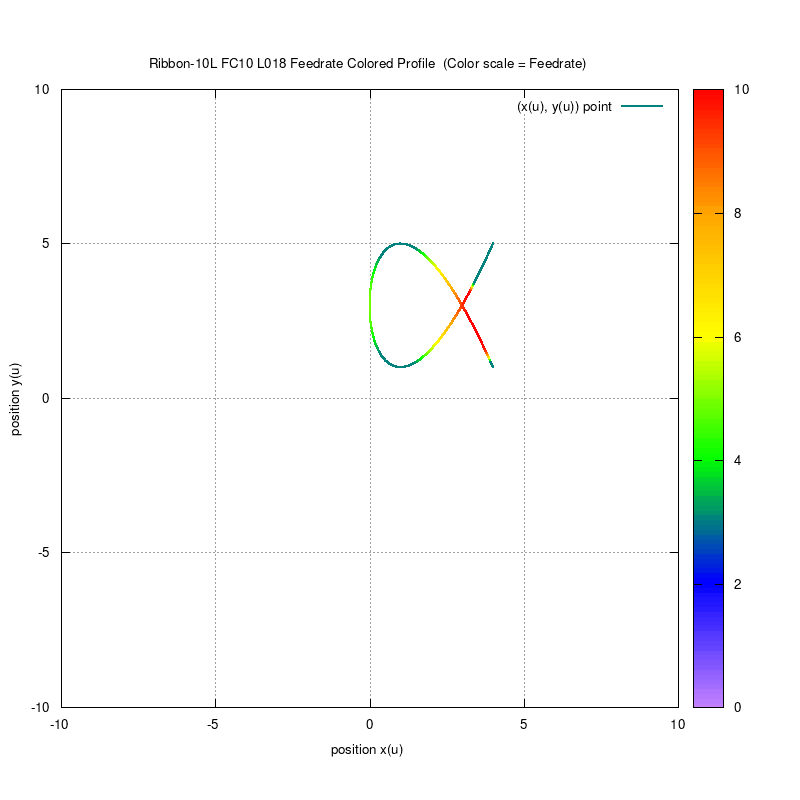
\includegraphics[width=0.75\textwidth]{Chap4/appendix/app-Ribbon-10L/plots/17-img-Ribbon-10L-FC10-Colored-Feedrate-Profile-data_ngcode.png}
\end{figure}


\begin{figure}
	\caption     {Ribbon-10L FC20 Colored Feedrate Profile data ngcode}
	\label{18-img-Ribbon-10L-FC20-Colored-Feedrate-Profile-data_ngcode.png}
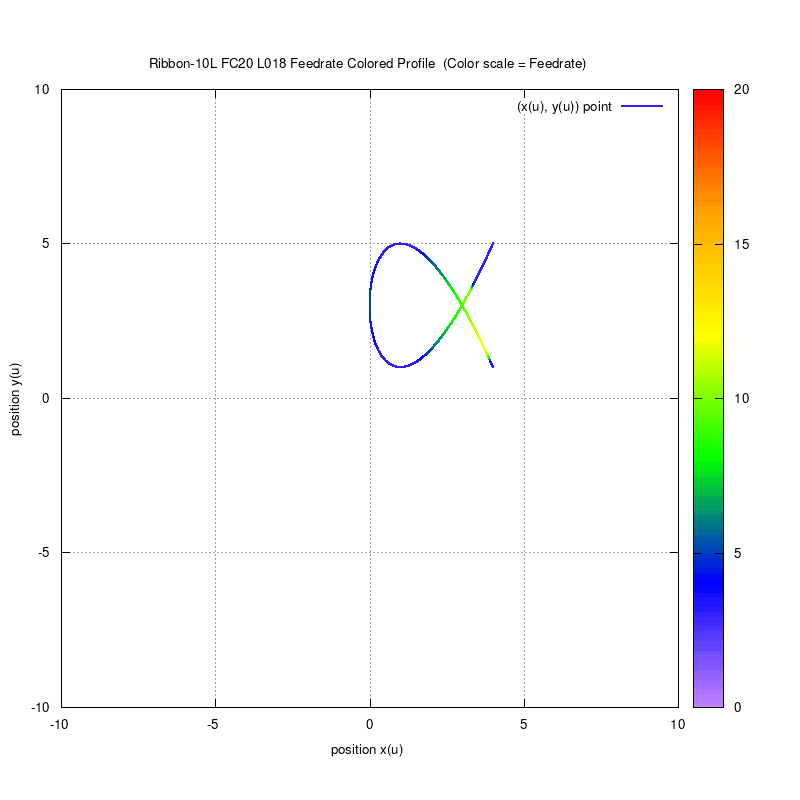
\includegraphics[width=0.75\textwidth]{Chap4/appendix/app-Ribbon-10L/plots/18-img-Ribbon-10L-FC20-Colored-Feedrate-Profile-data_ngcode.png}
\end{figure}

%% ==================================================
\clearpage
\pagebreak

\begin{figure}
	\caption     {Ribbon-10L FC30 Colored Feedrate Profile data ngcode}
	\label{19-img-Ribbon-10L-FC30-Colored-Feedrate-Profile-data_ngcode.png}
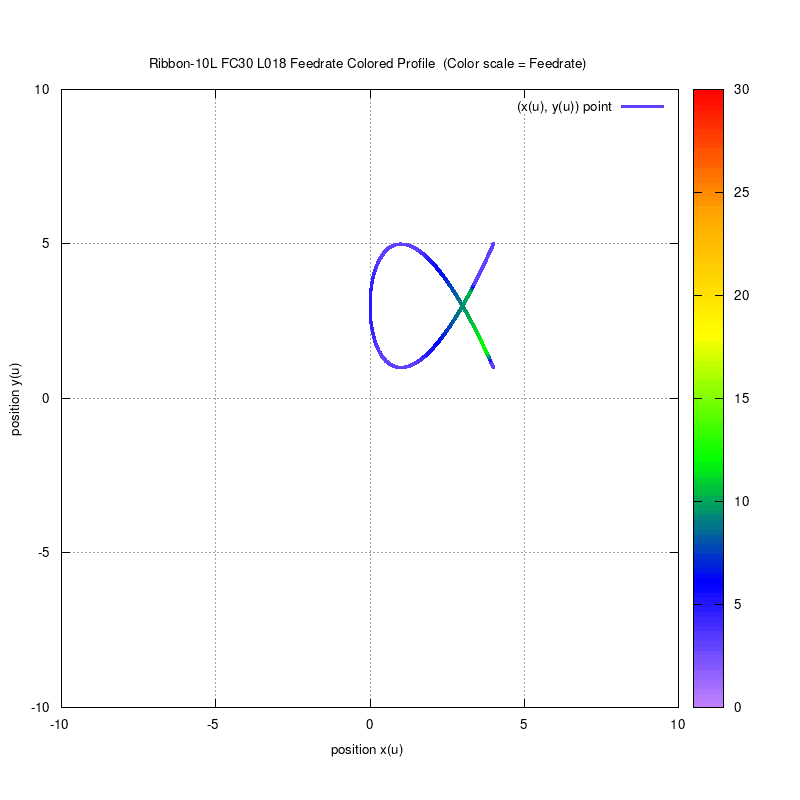
\includegraphics[width=0.75\textwidth]{Chap4/appendix/app-Ribbon-10L/plots/19-img-Ribbon-10L-FC30-Colored-Feedrate-Profile-data_ngcode.png}
\end{figure}


\begin{figure}
	\caption     {Ribbon-10L FC40 Colored Feedrate Profile data ngcode}
	\label{20-img-Ribbon-10L-FC40-Colored-Feedrate-Profile-data_ngcode.png}
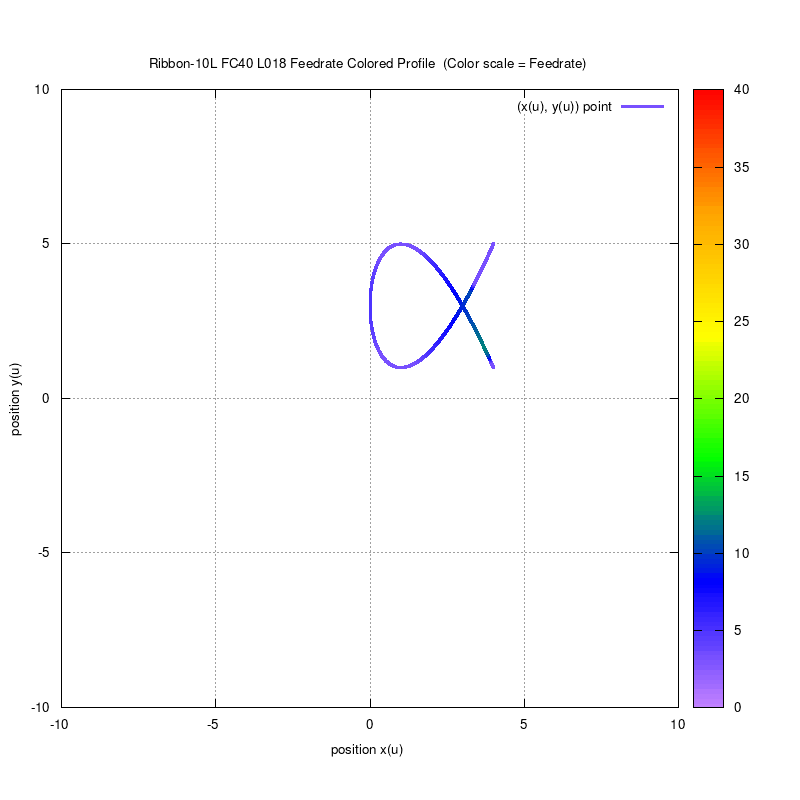
\includegraphics[width=0.75\textwidth]{Chap4/appendix/app-Ribbon-10L/plots/20-img-Ribbon-10L-FC40-Colored-Feedrate-Profile-data_ngcode.png}
\end{figure}

%% ==================================================
\clearpage
\pagebreak

\begin{figure}
	\caption     {Ribbon-10L FC10 Tangential Acceleration}
	\label{21-img-Ribbon-10L-FC10-Tangential-Acceleration.pdf}
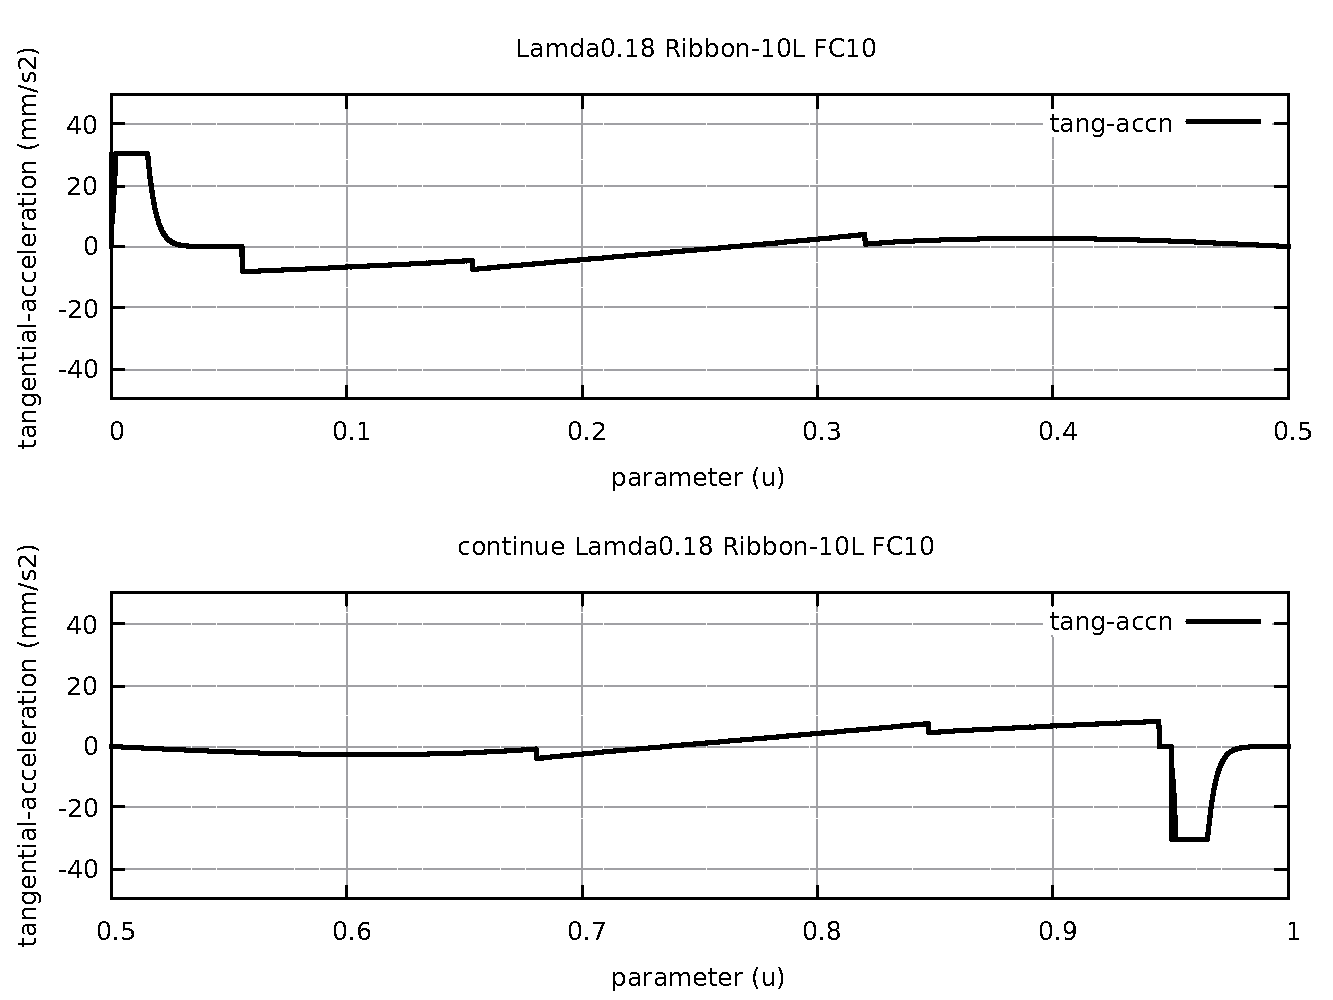
\includegraphics[width=1.00\textwidth]{Chap4/appendix/app-Ribbon-10L/plots/21-img-Ribbon-10L-FC10-Tangential-Acceleration.pdf}
\end{figure}


\begin{figure}
	\caption     {Ribbon-10L FC20 Tangential Acceleration}
	\label{22-img-Ribbon-10L-FC20-Tangential-Acceleration.pdf}
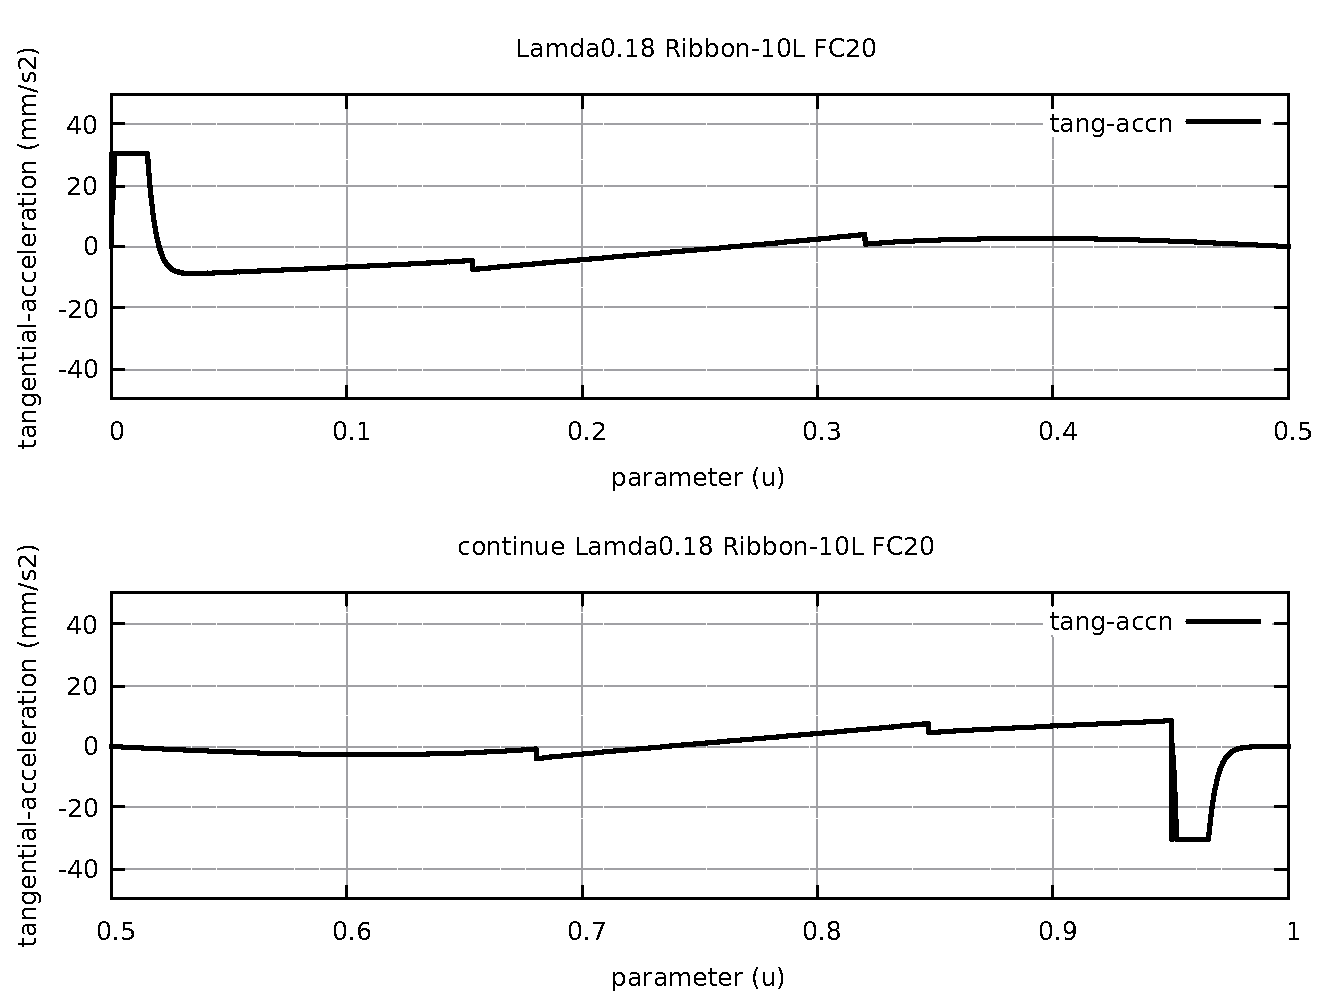
\includegraphics[width=1.00\textwidth]{Chap4/appendix/app-Ribbon-10L/plots/22-img-Ribbon-10L-FC20-Tangential-Acceleration.pdf}
\end{figure}

%% ==================================================
\clearpage
\pagebreak

\begin{figure}
	\caption     {Ribbon-10L FC30 Tangential Acceleration}
	\label{23-img-Ribbon-10L-FC30-Tangential-Acceleration.pdf}
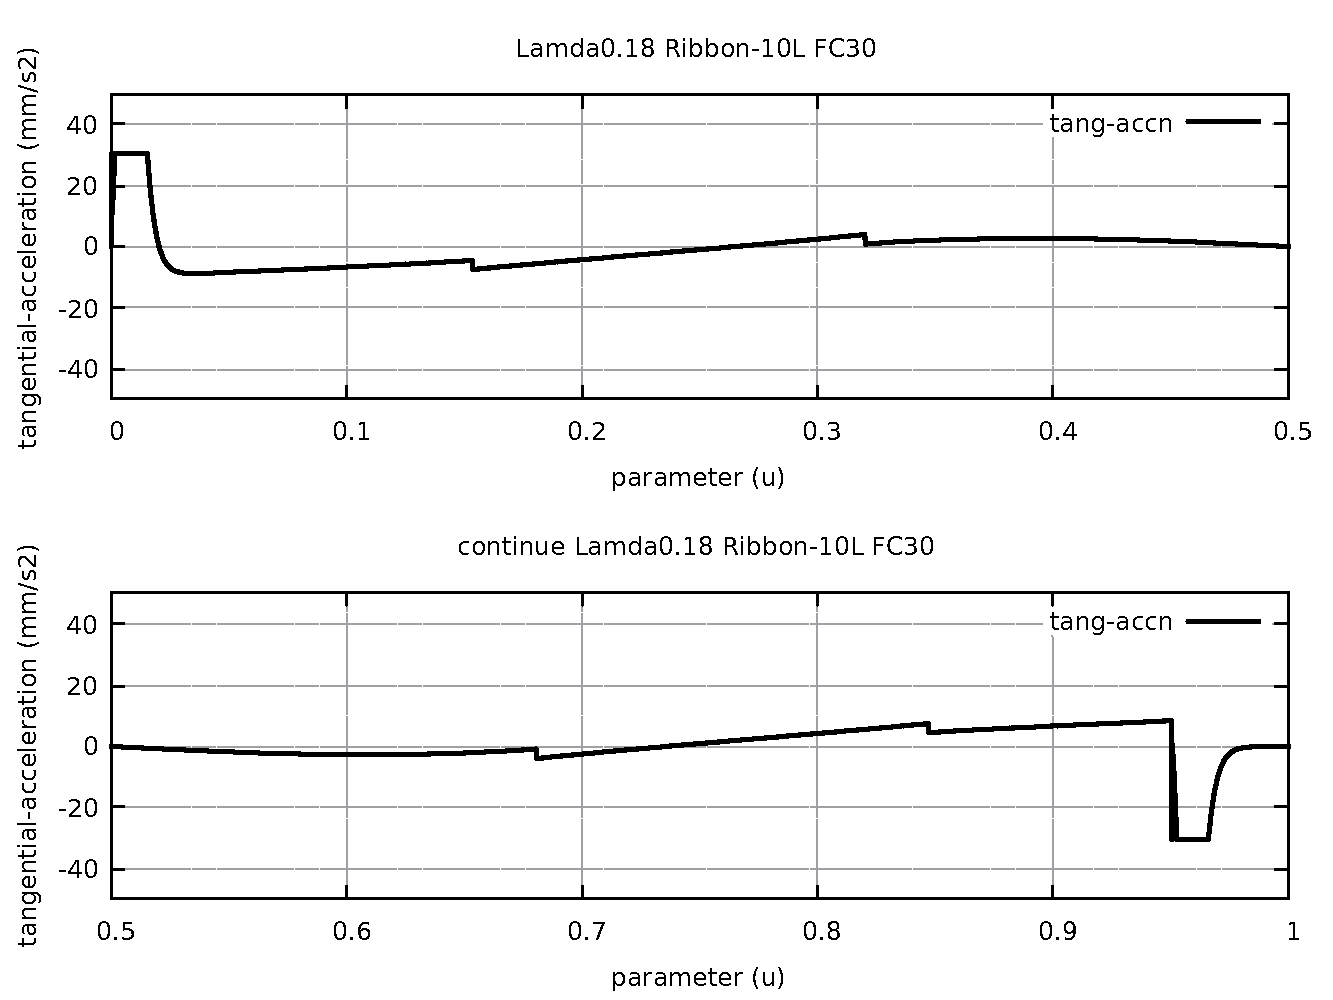
\includegraphics[width=1.00\textwidth]{Chap4/appendix/app-Ribbon-10L/plots/23-img-Ribbon-10L-FC30-Tangential-Acceleration.pdf}
\end{figure}


\begin{figure}
	\caption     {Ribbon-10L FC40 Tangential Acceleration}
	\label{24-img-Ribbon-10L-FC40-Tangential-Acceleration.pdf}
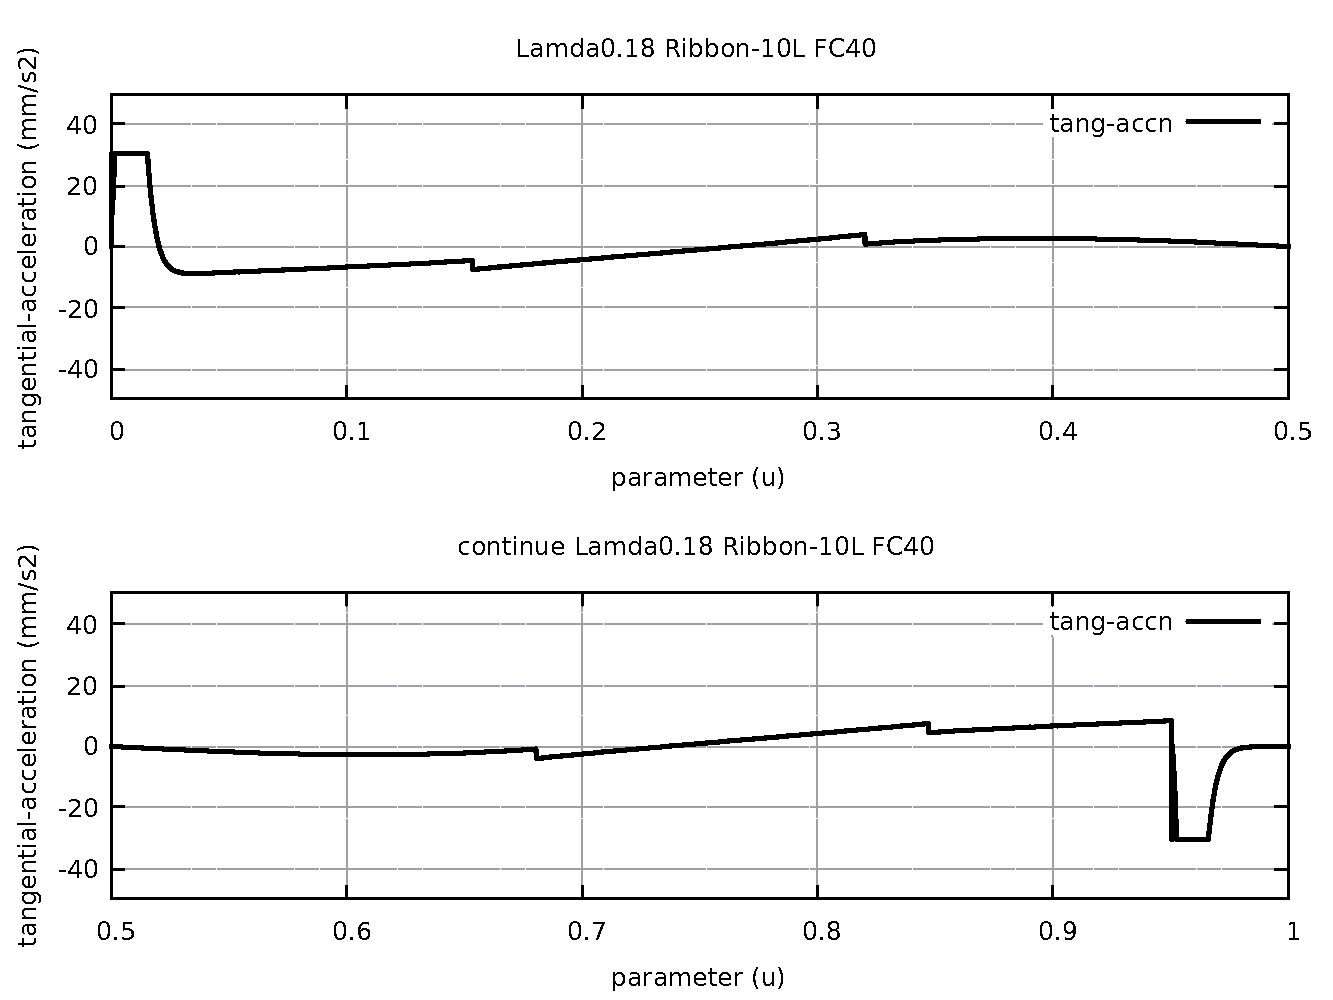
\includegraphics[width=1.00\textwidth]{Chap4/appendix/app-Ribbon-10L/plots/24-img-Ribbon-10L-FC40-Tangential-Acceleration.pdf}
\end{figure}

%% ==================================================
\clearpage
\pagebreak

\begin{figure}
	\caption     {Ribbon-10L FC20 Nominal Separation NAL and NCL}
	\label{25-img-Ribbon-10L-FC20-Nominal-Separation-NAL-and-NCL.pdf}
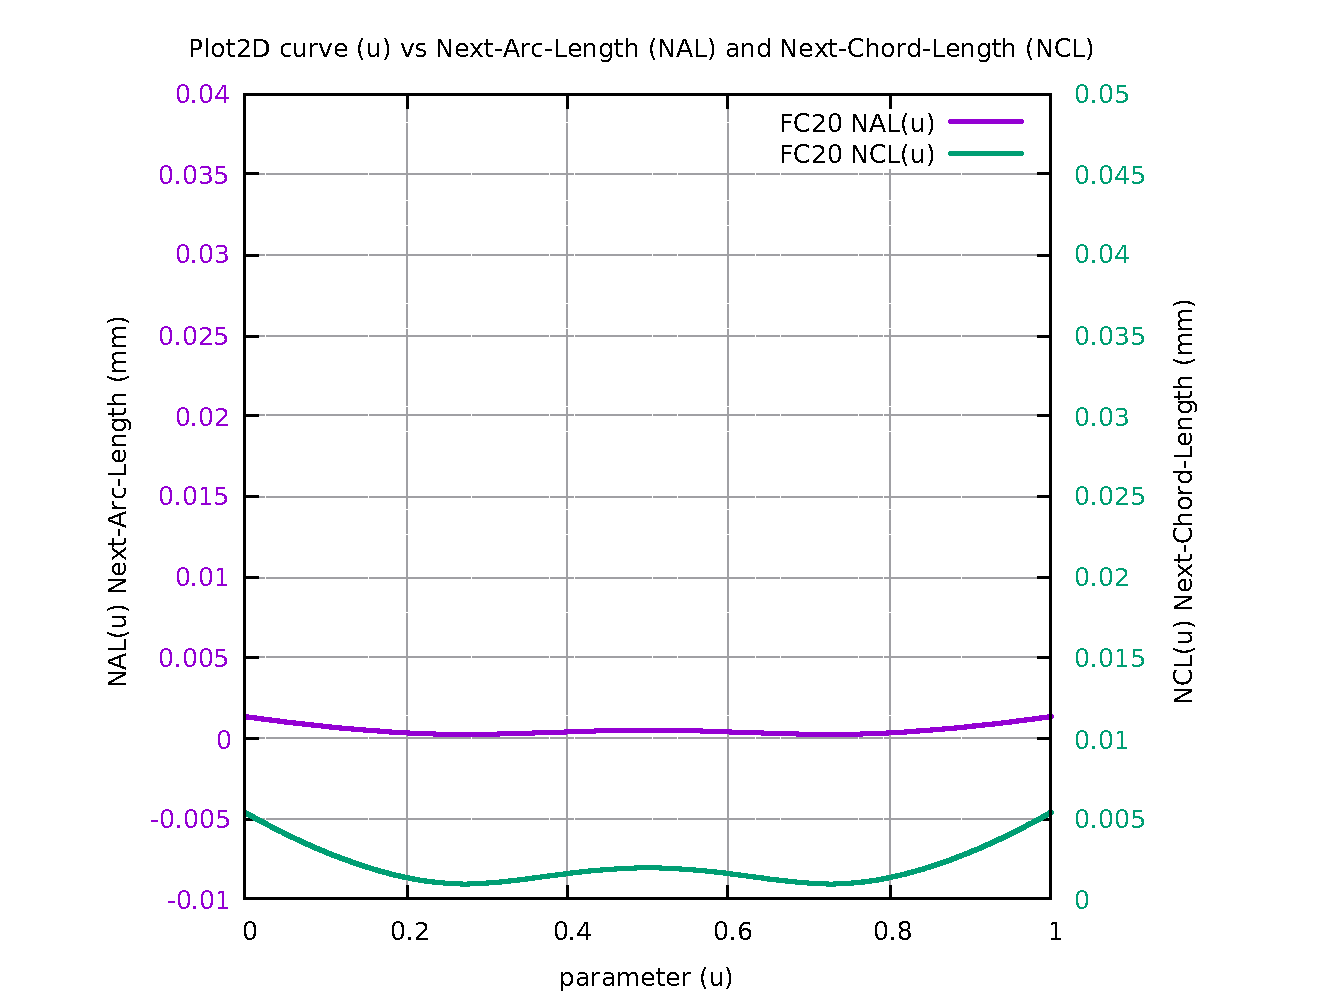
\includegraphics[width=1.00\textwidth]{Chap4/appendix/app-Ribbon-10L/plots/25-img-Ribbon-10L-FC20-Nominal-Separation-NAL-and-NCL.pdf}
\end{figure}


\begin{figure}
	\caption     {Ribbon-10L SAL minus SCL for FC10 FC20 FC30 FC40}
	\label{26-img-Ribbon-10L-SAL-minus-SCL-for-FC10-FC20-FC30-FC40.pdf}
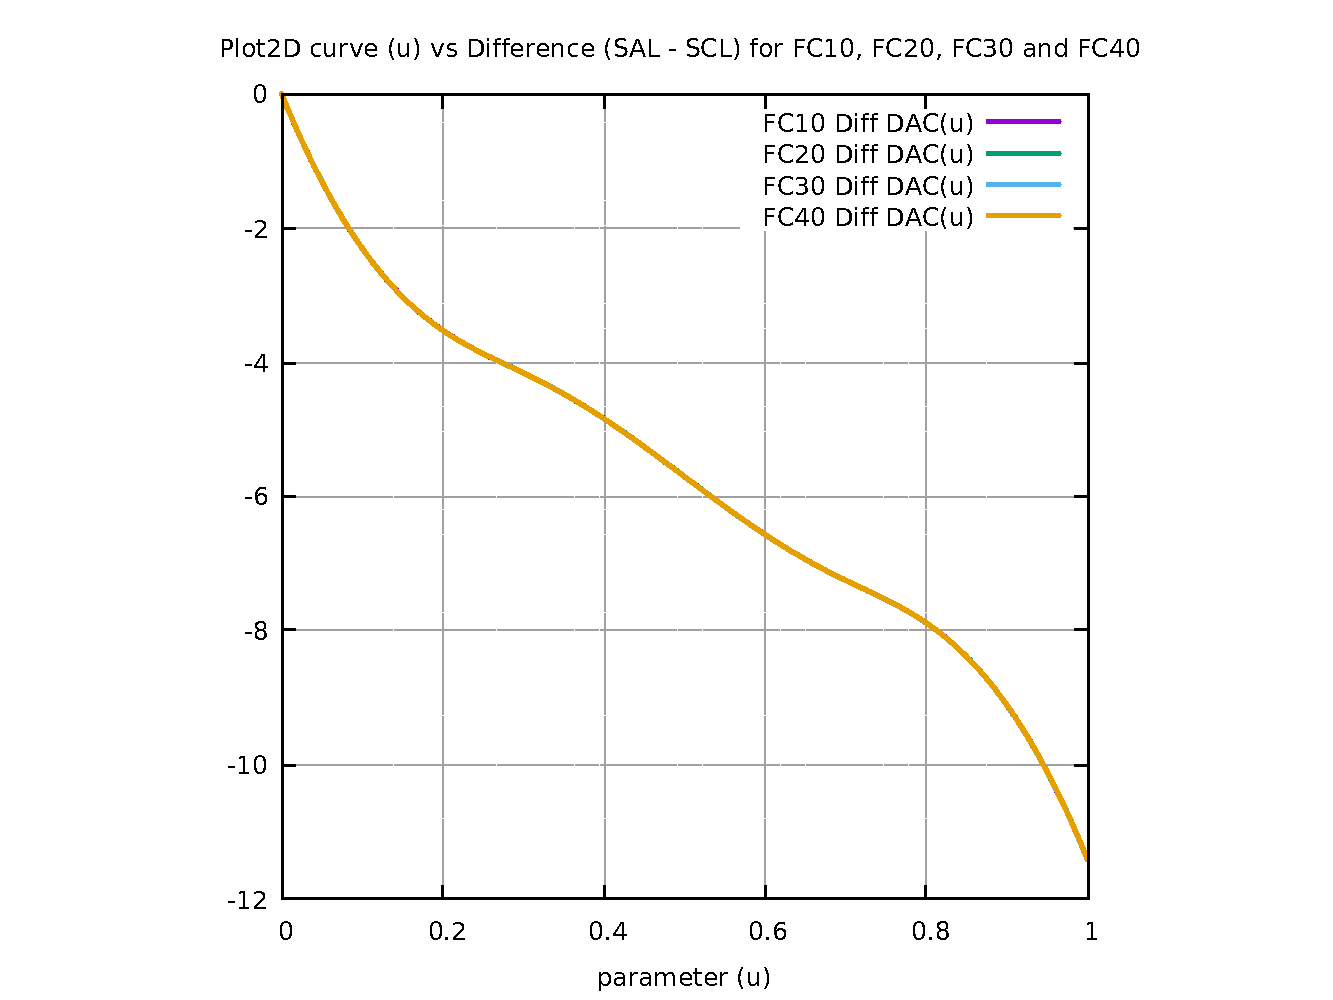
\includegraphics[width=1.00\textwidth]{Chap4/appendix/app-Ribbon-10L/plots/26-img-Ribbon-10L-Difference-SAL-minus-SCL-for-FC10-FC20-FC30-FC40.pdf}
\end{figure}


%% ==================================================
\clearpage
\pagebreak

\begin{figure}
	\caption     {Ribbon-10L FC10 FrateCmd CurrFrate X-Frate Y-Frate}
	\label{27-img-Ribbon-10L-FC10-FrateCmd-CurrFrate-X-Frate-Y-Frate.pdf}
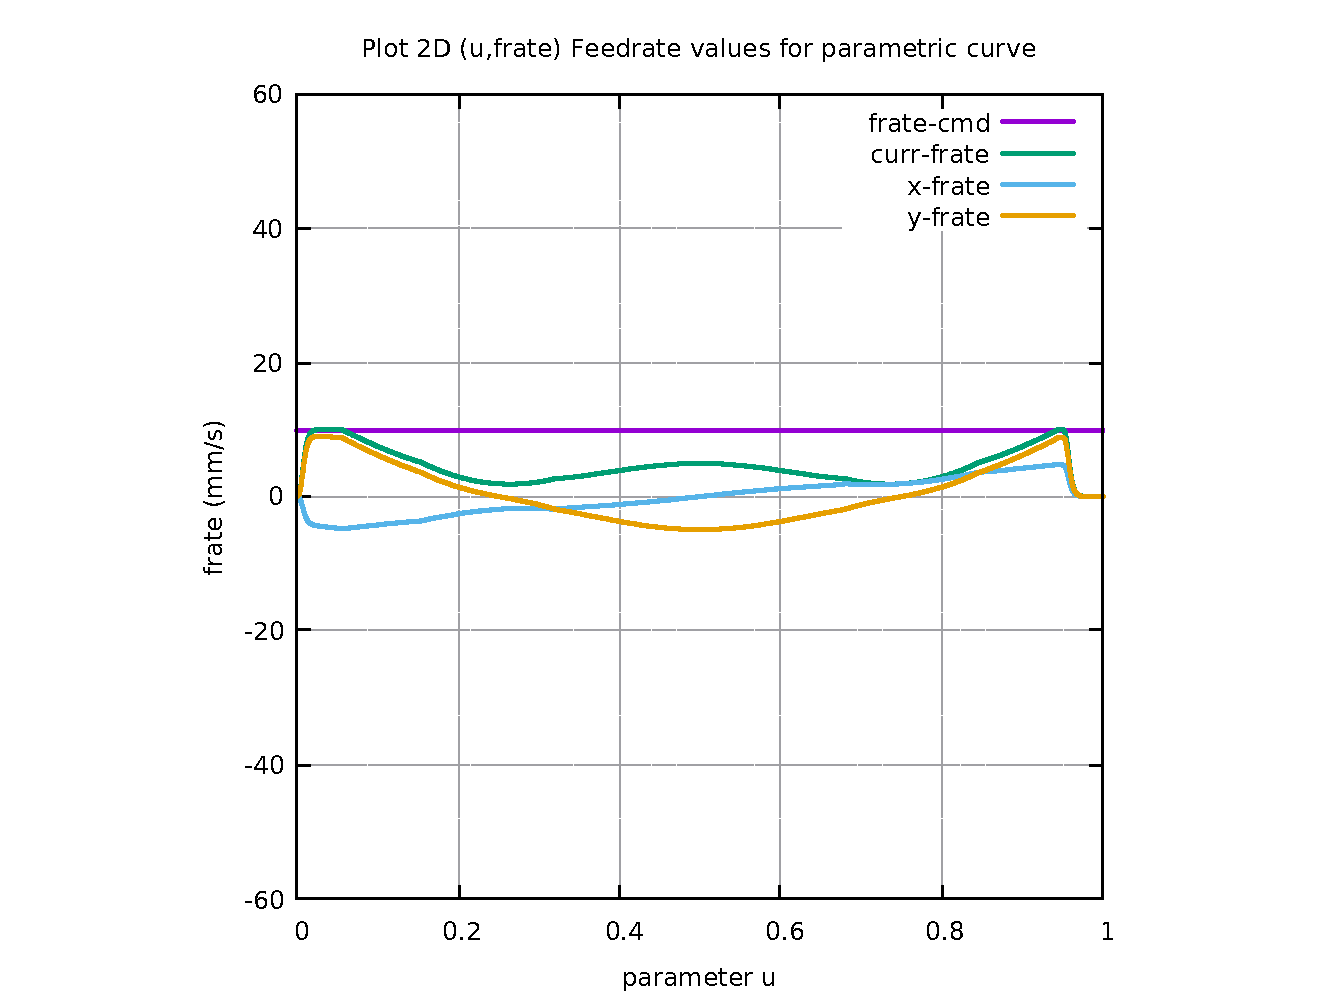
\includegraphics[width=1.00\textwidth]{Chap4/appendix/app-Ribbon-10L/plots/27-img-Ribbon-10L-FC10-FrateCmd-CurrFrate-X-Frate-Y-Frate.pdf}
\end{figure}


\begin{figure}
	\caption     {Ribbon-10L FC20 FrateCmd CurrFrate X-Frate Y-Frate}
	\label{28-img-Ribbon-10L-FC20-FrateCmd-CurrFrate-X-Frate-Y-Frate.pdf}
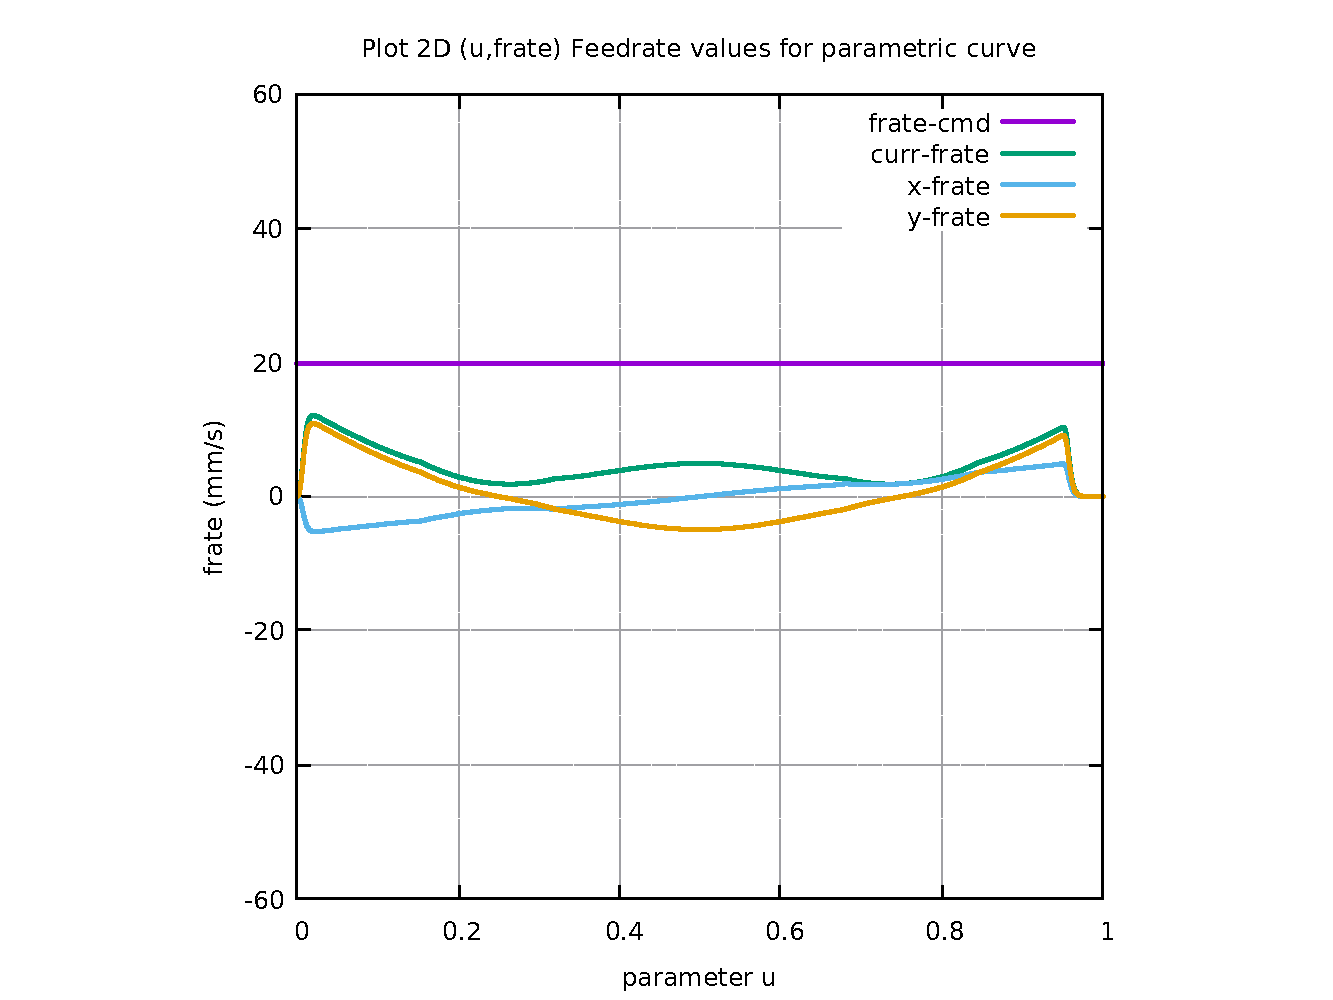
\includegraphics[width=1.00\textwidth]{Chap4/appendix/app-Ribbon-10L/plots/28-img-Ribbon-10L-FC20-FrateCmd-CurrFrate-X-Frate-Y-Frate.pdf}
\end{figure}


%% ==================================================
\clearpage
\pagebreak

\begin{figure}
	\caption     {Ribbon-10L FC30 FrateCmd CurrFrate X-Frate Y-Frate}
	\label{29-img-Ribbon-10L-FC30-FrateCmd-CurrFrate-X-Frate-Y-Frate.pdf}
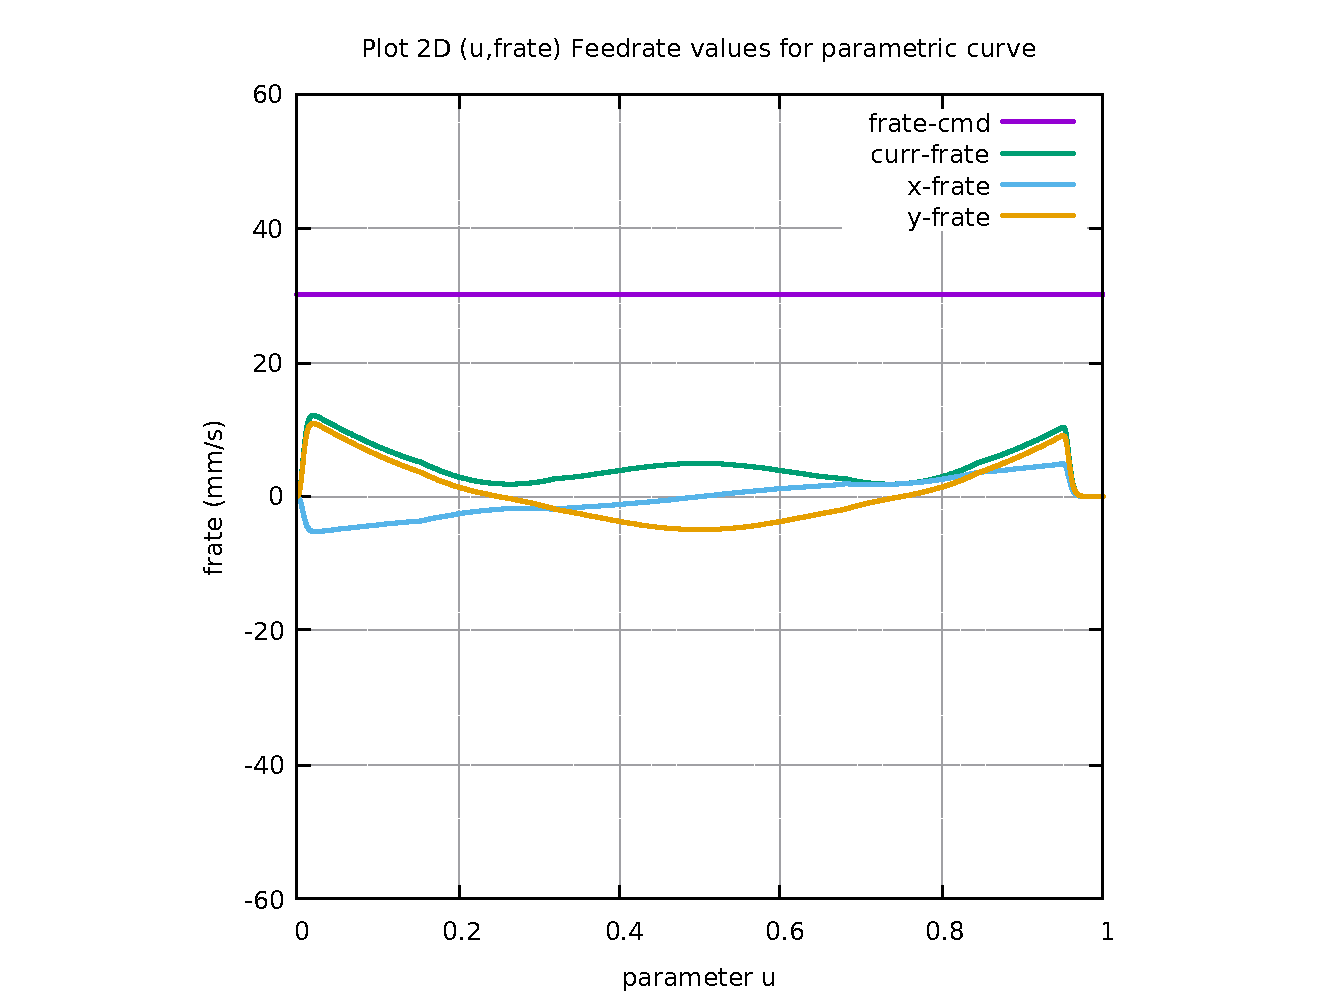
\includegraphics[width=1.00\textwidth]{Chap4/appendix/app-Ribbon-10L/plots/29-img-Ribbon-10L-FC30-FrateCmd-CurrFrate-X-Frate-Y-Frate.pdf}
\end{figure}


\begin{figure}
	\caption     {Ribbon-10L FC40 FrateCmd CurrFrate X-Frate Y-Frate}
	\label{30-img-Ribbon-10L-FC40-FrateCmd-CurrFrate-X-Frate-Y-Frate.pdf}
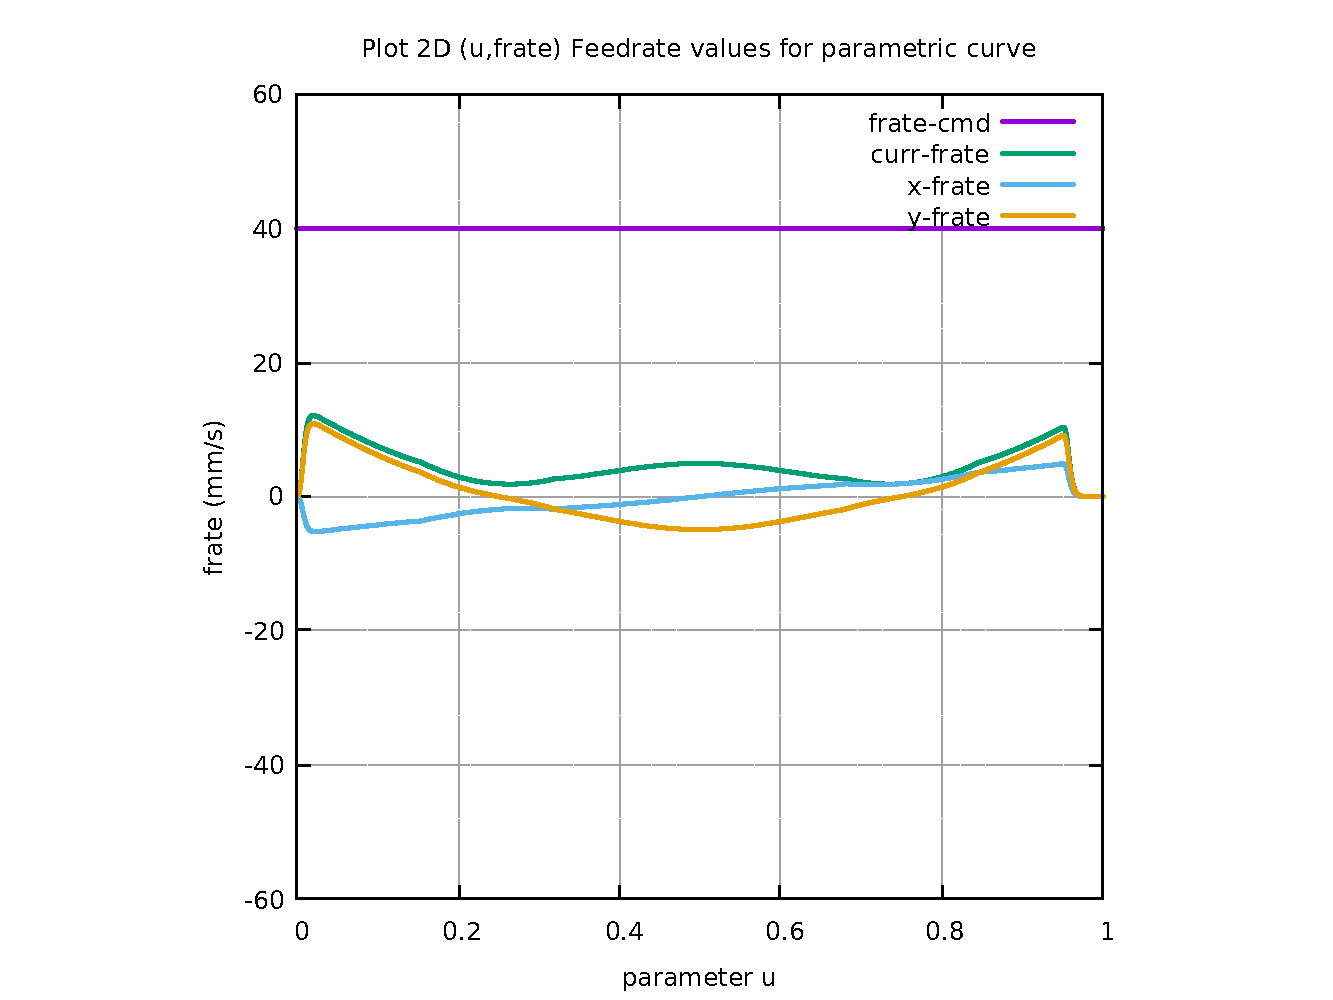
\includegraphics[width=1.00\textwidth]{Chap4/appendix/app-Ribbon-10L/plots/30-img-Ribbon-10L-FC40-FrateCmd-CurrFrate-X-Frate-Y-Frate.pdf}
\end{figure}


%% ==================================================
\clearpage
\pagebreak

\begin{figure}
	\caption     {Ribbon-10L FC10 Four Components FeedrateLimit}
	\label{31-img-Ribbon-10L-FC10-Four-Components-FeedrateLimit.pdf}
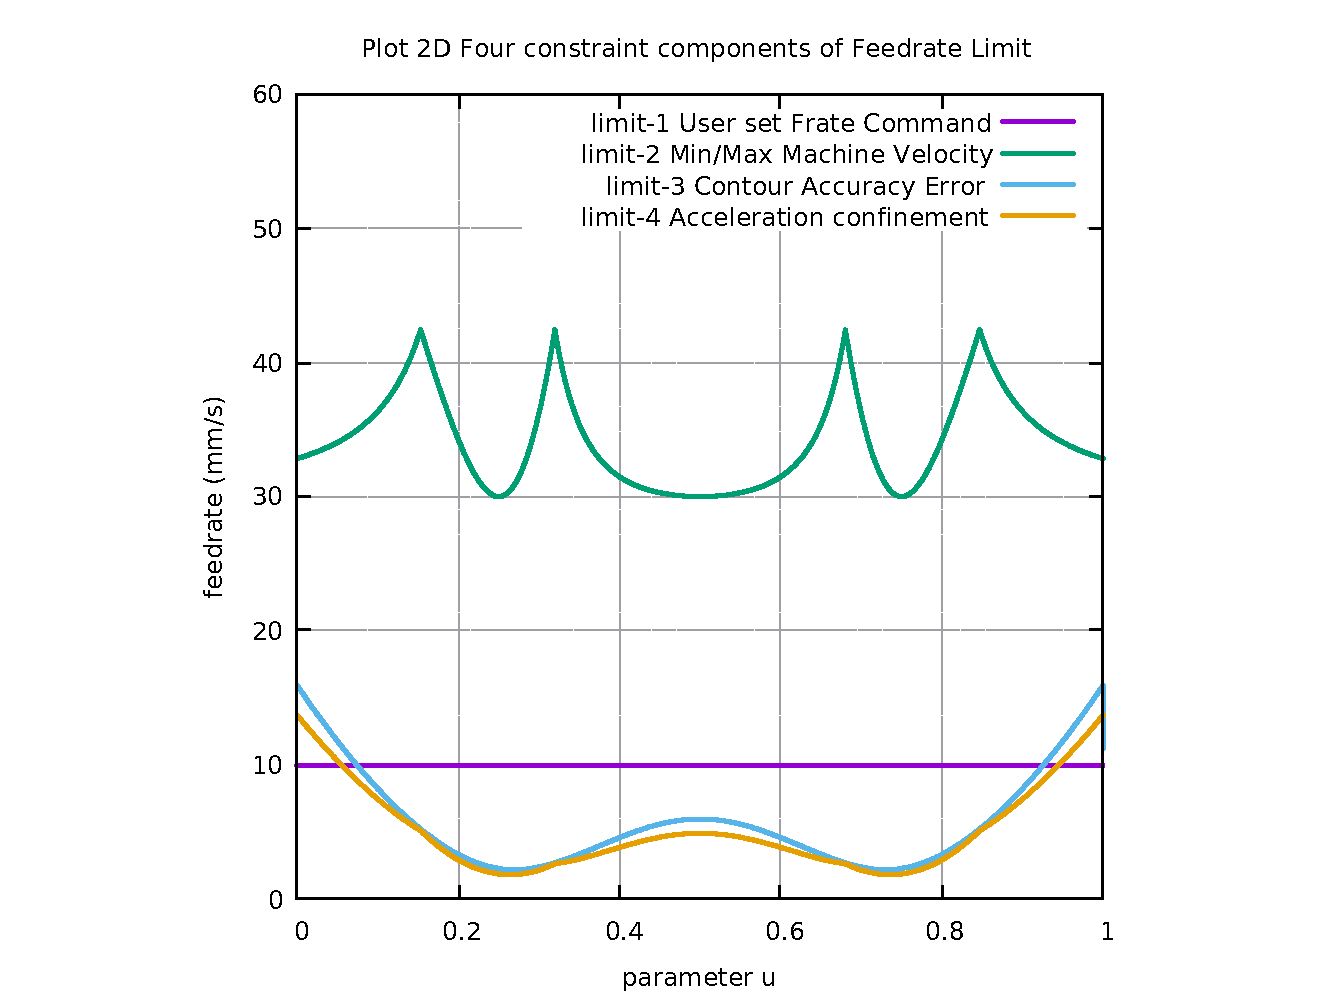
\includegraphics[width=1.00\textwidth]{Chap4/appendix/app-Ribbon-10L/plots/31-img-Ribbon-10L-FC10-Four-Components-FeedrateLimit.pdf}
\end{figure}


\begin{figure}
	\caption     {Ribbon-10L FC20 Four Components FeedrateLimit}
	\label{32-img-Ribbon-10L-FC20-Four-Components-FeedrateLimit.pdf}
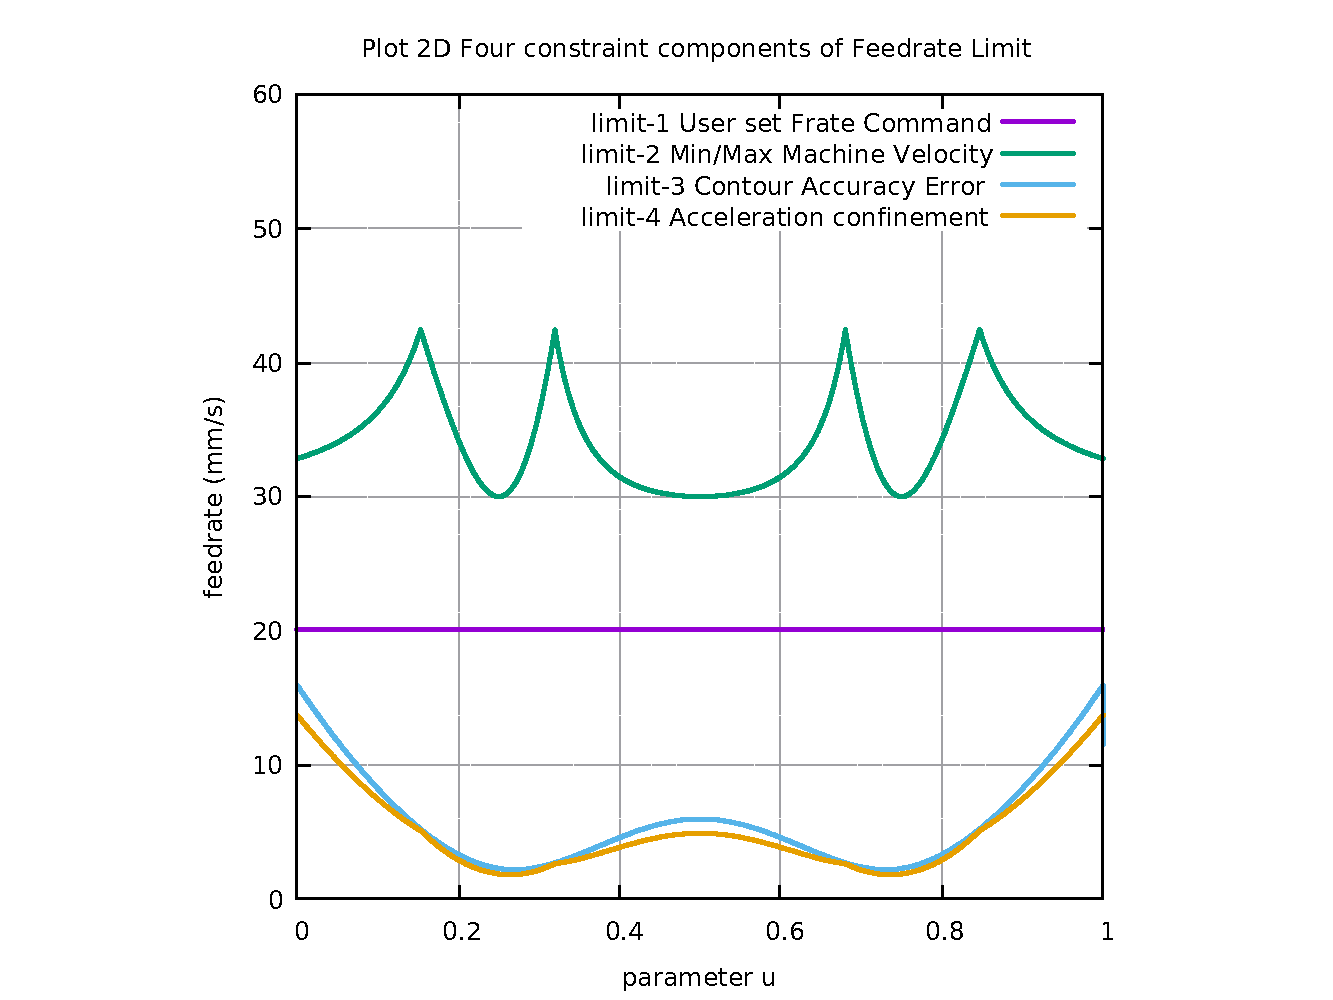
\includegraphics[width=1.00\textwidth]{Chap4/appendix/app-Ribbon-10L/plots/32-img-Ribbon-10L-FC20-Four-Components-FeedrateLimit.pdf}
\end{figure}


%% ==================================================
\clearpage
\pagebreak

\begin{figure}
	\caption     {Ribbon-10L FC30 Four Components FeedrateLimit}
	\label{33-img-Ribbon-10L-FC30-Four-Components-FeedrateLimit.pdf}
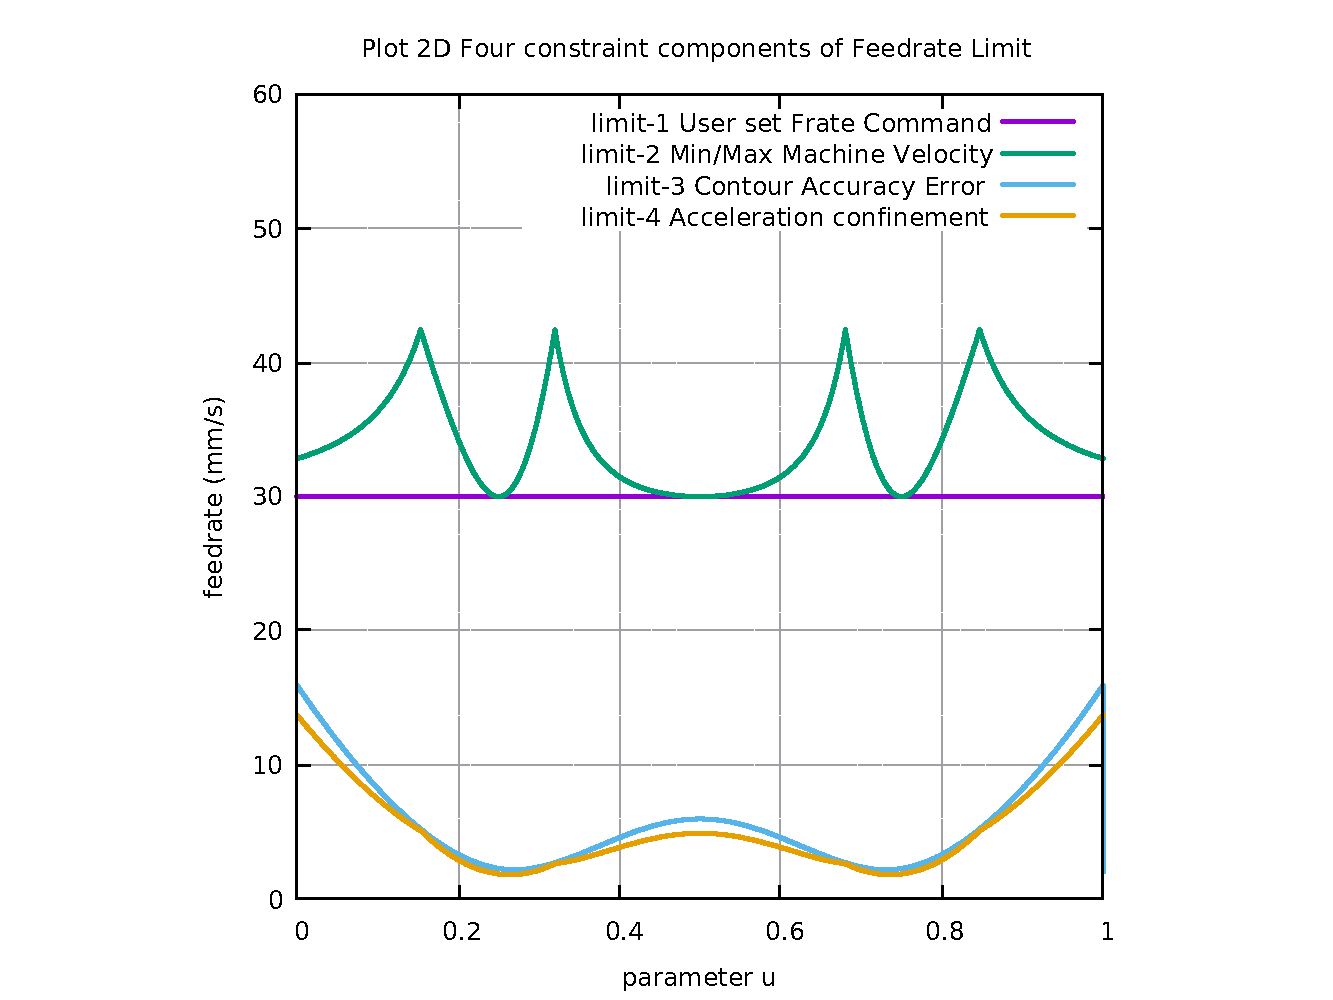
\includegraphics[width=1.00\textwidth]{Chap4/appendix/app-Ribbon-10L/plots/33-img-Ribbon-10L-FC30-Four-Components-FeedrateLimit.pdf}
\end{figure}


\begin{figure}
	\caption     {Ribbon-10L FC40 Four Components FeedrateLimit}
	\label{34-img-Ribbon-10L-FC40-Four-Components-FeedrateLimit.pdf}
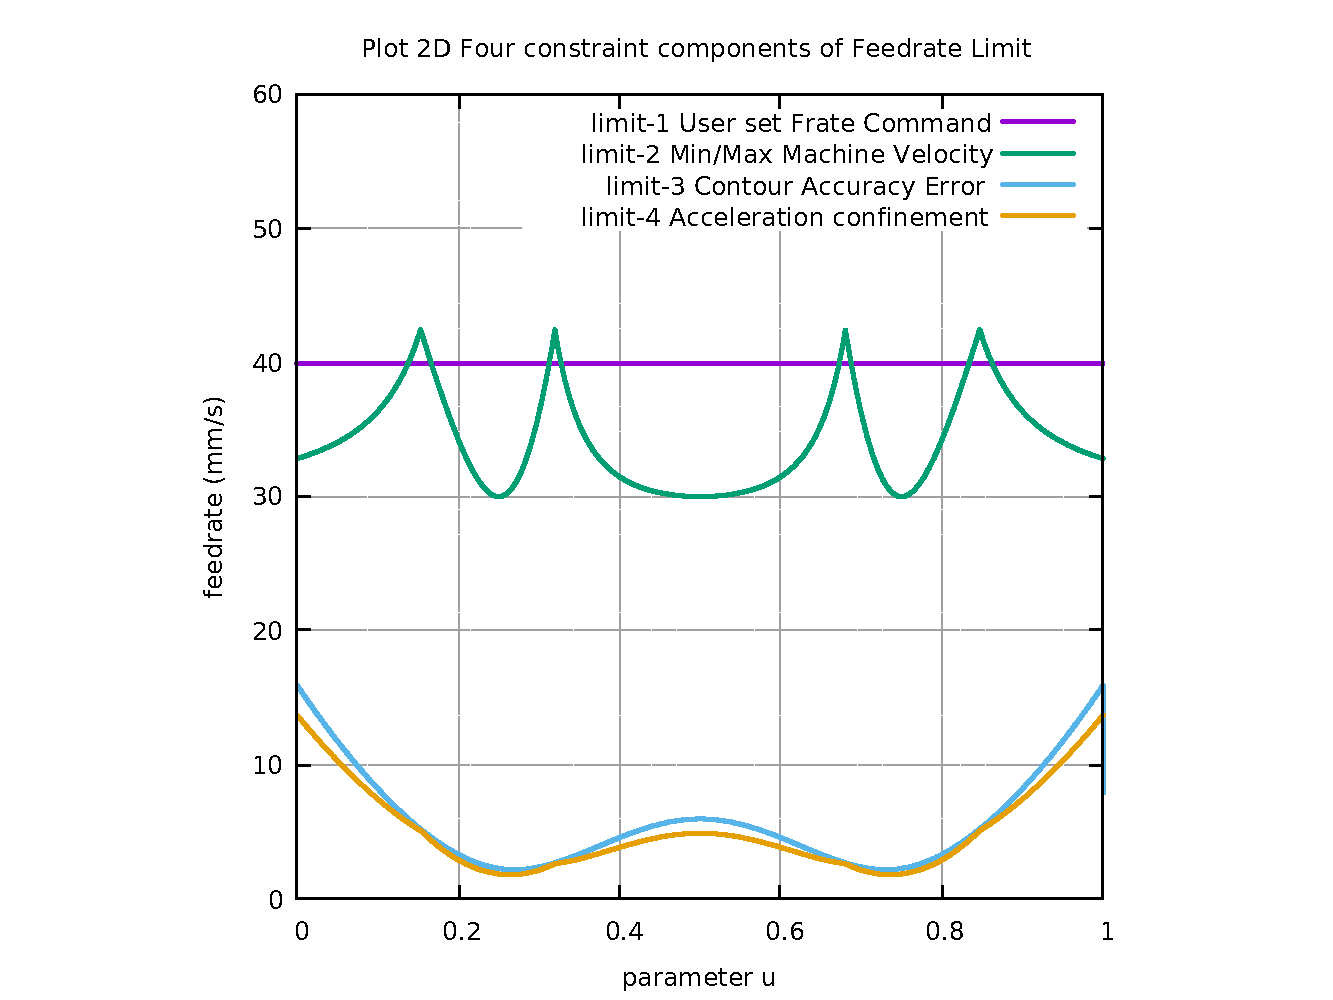
\includegraphics[width=1.00\textwidth]{Chap4/appendix/app-Ribbon-10L/plots/34-img-Ribbon-10L-FC40-Four-Components-FeedrateLimit.pdf}
\end{figure}


%% =======================================
\clearpage
\pagebreak

\begin{figure}
	\centering
	\caption     {Ribbon-10L Histogram Points FC10 FC20 FC30 FC40}
	\label{35-img-Ribbon-10L-Histogram-Points-FC10-FC20-FC30-FC40.pdf}
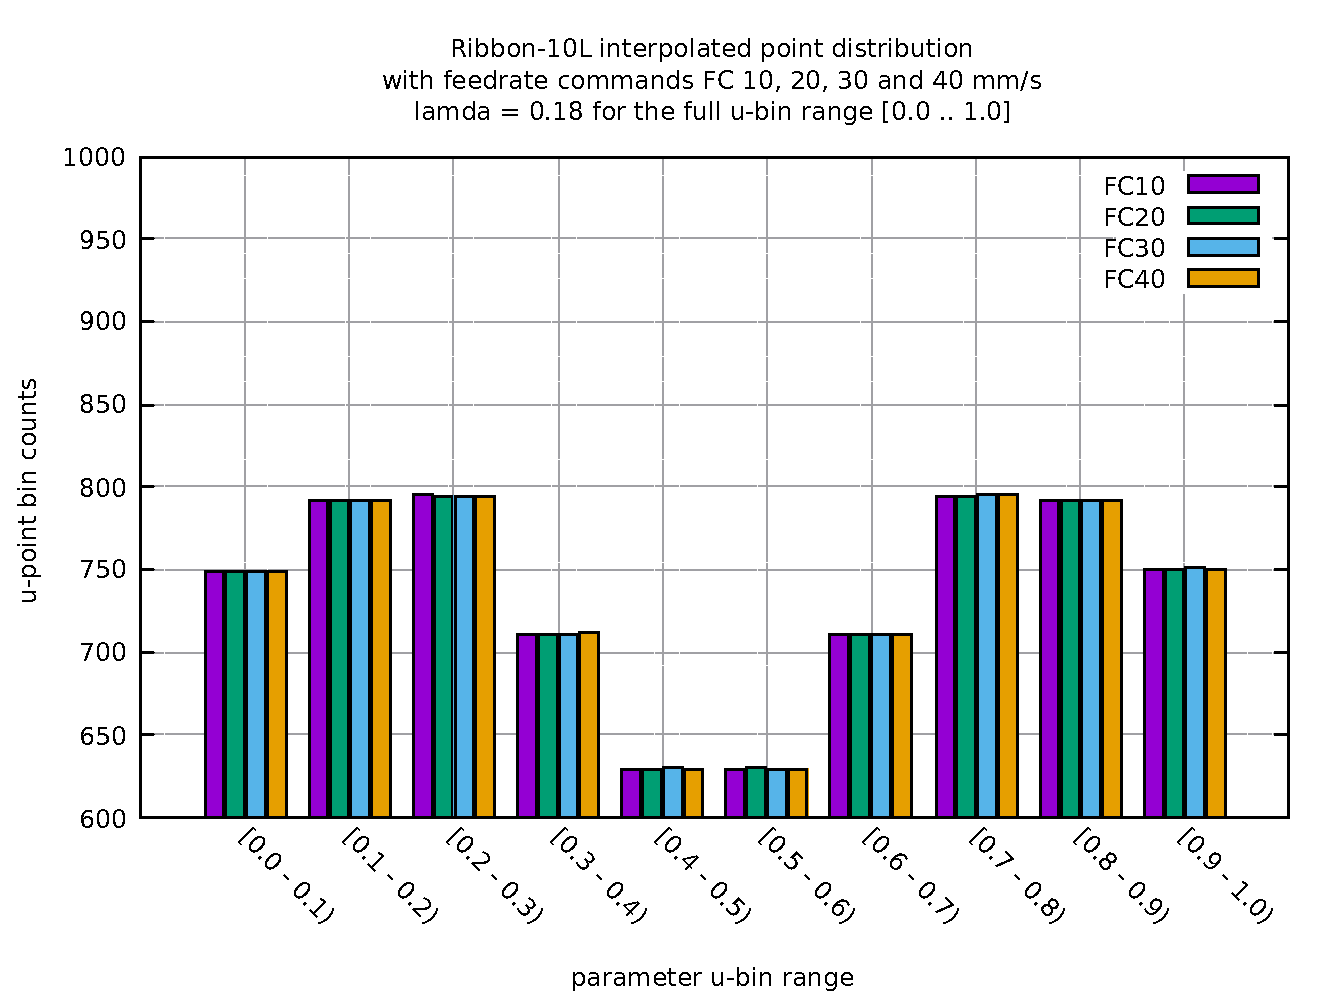
\includegraphics[width=1.00\textwidth]{Chap4/appendix/app-Ribbon-10L/plots/35-img-Ribbon-10L-Histogram-Points-FC10-FC20-FC30-FC40.pdf} 
\end{figure}


\begin{table}[ht]
%% \begin{center}
\caption    {Ribbon-10L Table distribution of interpolated points}
\label  {tab-Ribbon-10L Table distribution of interpolated points}
	
%% IMPORTANT TO SCALEBOX BELOW
\scalebox{0.80}{
		
%% START COPY AND PASTE BELOW HERE
%% FROM \begin{tabular} UNTIL \end{tabular)
%% Note: adjust last p{} to get line width correct
		
\begin{tabular}{ p{4.5cm} p{1.5cm} p{1.5cm} p{1.5cm} p{7.50cm} }
\hline
	&		&		&		&		\\
BINS	&	FC10	&	FC20	&	FC30	&	FC40	\\
&		&		&		&		\\
0.0 - 0.1	&	749	&	749	&	749	&	749	\\
0.1 - 0.2	&	791	&	792	&	792	&	792	\\
0.2 - 0.3	&	795	&	794	&	794	&	794	\\
0.3 - 0.4	&	711	&	711	&	711	&	712	\\
0.4 - 0.5	&	629	&	629	&	630	&	629	\\
0.5 - 0.6	&	629	&	630	&	629	&	629	\\
0.6 - 0.7	&	711	&	711	&	711	&	711	\\
0.7 - 0.8	&	794	&	794	&	795	&	795	\\
0.8 - 0.9	&	792	&	792	&	791	&	792	\\
0.9 - 1.0	&	750	&	750	&	751	&	750	\\
&		&		&		&		\\
Tot Counts	&	7351	&	7352	&	7353	&	7353	\\
&		&		&		&		\\
\hline	
\end{tabular}
		
%% END COPY AND PASTE ABOVE HERE
		
}   %% IMPORTANT FOR SCALEBOX CLOSING
	
\end{table}
%% \end{landscape}

%% Ribbon-10L SUMMARY TABLE
%% ========================================================
\clearpage
\pagebreak
\begin{landscape}
	
\begin{table}[ht]
%% \begin{center}
\caption       {Ribbon-10L Table FC10-20-30-40 Run Performance data}
\label{tab-app4-Ribbon-10L-Table-FC10-20-30-40-Run-Performance-data}
		
%% IMPORTANT TO SCALEBOX BELOW
\scalebox{0.90}{
			
%% START COPY AND PASTE BELOW HERE
%% FROM \begin{tabular} UNTIL \end{tabular)
			
\begin{tabular}{ p{0.2cm} p{8.80cm} p{4.00cm} p{4.0cm} p{4.00cm} p{4.0cm}}
	\hline
	&		&		&		&		&		\\
	1	&	Curve Type	&	RIBBON-10L	&	RIBBON-10L	&	RIBBON-10L	&	RIBBON-10L	\\
	2	&	User Feedrate Command FC(mm/s)                   	&	FC10	&	FC20	&	FC30	&	FC40	\\
	3	&	User Lamda Acceleration Safety Factor	&	0.18	&	0.18	&	0.18	&	0.18	\\
	&		&		&		&		&		\\
	4	&	Total Iterpolated Points (TIP)	&	7351	&	7352	&	7353	&	7353	\\
	5	&	Total Sum-Chord-Error (SCE) (mm)	&	7.331686925442E-03	&	7.330650001960E-03	&	7.330843544266E-03	&	7.330107781796E-03	\\
	6	&	Ratio 1 = (SCE/TIP) = Chord-Error/Point	&	9.975084252302E-07	&	9.972316694273E-07	&	9.971223536814E-07	&	9.970222771758E-07	\\
	&		&		&		&		&		\\
	7	&	Total Sum-Arc-Length (SAL) (mm)	&	3.802699021307E+00	&	3.802672335504E+00	&	3.803478267930E+00	&	3.802978777888E+00	\\
	8	&	Total Sum-Chord-Length (SCL) (mm)	&	1.521079586306E+01	&	1.521068903483E+01	&	1.521391385441E+01	&	1.521191524702E+01	\\
	9	&	Difference = (SAL – SCL) (mm)	&	-1.140809684176E+01	&	-1.140801669932E+01	&	-1.141043558648E+01	&	-1.140893646914E+01	\\
	10	&	Percentage Difference = (SAL – SCL)/SAL	&	-2.999999941577E+02	&	-2.999999919218E+02	&	-3.000000205782E+02	&	-3.000000035623E+02	\\
	&		&		&		&		&		\\
	11	&	Ratio 2 = (SCE/SCL) = Chord Error/Chord-Length	&	4.820054776519E-04	&	4.819406921788E-04	&	4.818512589475E-04	&	4.818661991448E-04	\\
	&		&		&		&		&		\\
	12	&	Total Sum-Arc-Theta (SAT) (rad)	&	5.446619853644E+00	&	5.446616685362E+00	&	5.446717935311E+00	&	5.446655391021E+00	\\
	13	&	Total Sum-Arc-Area (SAA) (mm2)	&	1.338515095667E-06	&	1.338121185915E-06	&	1.338217831316E-06	&	1.337920946871E-06	\\
	&		&		&		&		&		\\
	14	&	Ratio 3 = (SAA/SCL) = Arc-Area/Chord-Length	&	4.820054776519E-04	&	4.819406921788E-04	&	4.818512589475E-04	&	4.818661991448E-04	\\
	&		&		&		&		&		\\
	15	&	Average-Chord-Error (ACE) (mm)	&	9.975084252302E-07	&	9.972316694273E-07	&	9.971223536814E-07	&	9.970222771758E-07	\\
	16	&	Average-Arc-Length (AAL) (mm)	&	5.173740165044E-04	&	5.173000048298E-04	&	5.173392638643E-04	&	5.172713245223E-04	\\
	17	&	Average-Chord-Length (ACL) (mm)	&	2.069496035791E-03	&	2.069199977531E-03	&	2.069357161916E-03	&	2.069085316516E-03	\\
	18	&	Average-Arc-Theta (AAT) (rad)	&	7.410367147815E-04	&	7.409354761749E-04	&	7.408484678062E-04	&	7.408399606938E-04	\\
	19	&	Average-Arc-Area (AAA) (mm2)	&	1.821108973696E-10	&	1.820325378744E-10	&	1.820209237372E-10	&	1.819805422838E-10	\\
	&		&		&		&		&		\\
	20	&	Algorithm actual runtime on computer (ART) (s) 	&	65.683135834	&	59.539855092	&	75.452534184	&	73.307374778	\\
	&		&		&		&		&	\\	
	\hline
\end{tabular}

			
%% END COPY AND PASTE		
}   %% IMPORTANT FOR SCALEBOX CLOSING
		
\end{table}
\end{landscape}

%% =======================================
\clearpage
\pagebreak
